\documentclass[letter, 12pt]{article}

% Police, caractères spéciaux
\usepackage[utf8]{inputenc}
\usepackage[english]{babel}
\usepackage[T1]{fontenc}
\usepackage{amsmath, amssymb}
\usepackage{mathrsfs}
\usepackage{braket}

% Environnements, figures
\usepackage{graphicx}
\usepackage{caption}  % Pour avoir du contrôle sur la taille des titres
\usepackage{subcaption}  % Sous-figures
\usepackage{booktabs}  % Plus beaux tableaux
\usepackage{multirow}
\usepackage{hyperref}
%\usepackage{appendix}  % Pour avoir du contrôle sur les annexes
%\usepackage{tikz}
%\usepackage{float}
%\usepackage{array}

% Bibliographie
\usepackage[
    backend=biber,
    style=numeric, 
    citestyle=numeric,  %authoryear, 
    natbib=true,
    url=false, 
    doi=false,
    eprint=false, 
    isbn=false, 
    sorting=none, 
    maxnames=2
]{biblatex}
\usepackage{csquotes}
\bibliography{olfaction_neurosci}
% Enlever les "notes" exportées par Zotero (qui donnent le "publisher" par exemple)
\AtEveryBibitem{%
  \clearfield{note}
  \clearlist{language}%
}

% Enlever le "In:" inutile
\renewbibmacro{in:}{}

% Mise en page
\usepackage[left = 2.5cm, right = 2.5cm, top = 2.5cm, bottom = 2.5cm]{geometry}
\oddsidemargin=0mm
\evensidemargin=0mm
\parindent=0mm
\parskip=12pt plus 1pt minus 1pt
%\usepackage{setspace}  % Si on veut changer l'interligne
%\widowpenalty10000  % Pour éviter les lignes orphelines
%\clubpenalty10000


% Titres et sous-titres
\usepackage[pagestyles]{titlesec}
\titlespacing{\section}{0mm}{0pt}{0pt}
\captionsetup[figure]{font=small}  % Pour que le titre des figures soit plus petit

% Titres de sections  -> Changer après la table des matières seulement
\titleformat{\section}
{\large\normalfont\bfseries}
{\thesection}{0.1em}{. }
% Solution for numberless sections from https://tex.stackexchange.com/questions/102116/titlesec-and-section-in-titleformat
\titleformat{name=\section,numberless}[block]{\large\normalfont\bfseries}{}{0em}{}[]% starred version


% Titres de sous-sections
\titleformat{\subsection}
{\normalfont\bfseries}
{\thesubsection}{0.1em}{ }

% Nouvelles commandes et raccourcis
\def\tb{\textbf} 
\def\mb{\mathbf}
\newcommand{\prob}[1]{\mathbb{P}\left[ #1 \right]}
\newcommand{\card}[1]{\mathrm{card}\left( #1 \right)}
\newcommand{\esper}[1]{\mathbb{E}\left[ #1 \right]}
\newcommand{\variance}[1]{\mathrm{Var}\left[ #1 \right]}
\def\beq{ \begin{equation} }		% \beq remplace maintenant \begin{equation}	
\def\eeq{ \end{equation} } 			% \eeq remplace maintenant \end{equation}
\def\ovl{\overline}
\def\avgnu{\braket{\nu}}


\title{Notes on the IBCM model for olfactory background inhibition}
\author{François Bourassa}
\date{\today}

\begin{document}
\maketitle

{\parskip=1pt plus 1pt minus 1pt
\tableofcontents
}
\parskip=12pt plus 1pt minus 1pt

% Summary of the goal and model chosen. A few sentences, not more. Like an abstract, but only of the technical part. 
\section{Introduction}
\label{sect:introduction}
% I just tried writing an introduction for myself. Let's keep this shorter as these are notes for collaborators. 
%From insects to mammals, organisms navigate complex olfactory landscapes by picking up new odors amidst fluctuating mixtures of irrelevant background odorants. Habituation to the olfactory background on the time scale of an hour is thought to help organisms discriminate the appearance of relevant odors in the olfactory landscape \cite{shen_habituation_2020}. Habituation has been shown to occur in \textit{Drosophila} due to interneuron plasticity \cite{das_plasticity_2011}, and the ability of \textit{Lepidoptera} species (moths) to pick out exquisite trails of pheromones in turbulent environments brimming with odoriferous sources indicates that the phenomenon is general. This background habituation task, related to figure-ground segregation problems, is a non-trivial statistical problem, but it is unclear how this problem is solved in the olfactory cortex of those various organisms. 
% Would need more, better examples of habituation. 

% Very short introduction
A broad variety of organisms are able to habituate to fluctuating olfactory background, thus enhancing their ability  and to recognize new odors that appear. The neural mechanisms enabling this habituation to fluctuating mixtures are not well understood but are of interest for the broad problem of figure-background segregation in time-varying signals. 

An olfactory network model implementing a simple habituation algorithm has been proposed recently \cite{shen_habituation_2020}. It achieves subtraction of the average background: post-habituation recognition of new odors improves when the background is constant, but performance is lost against fluctuating backgrounds. A more sophisticated neural mechanism is needed to achieve efficient habituation. %, to suppress fluctuations of the background as well as its average. 

The IBCM model of neural plasticity is a promising avenue to account for olfactory habituation. In this model, neurons become responsive specifically to certain components of the stimuli to which they are exposed. 
%Fluctuations of the stimuli actually drive neurons to respond to non-Gaussian projections of the input distribution.
The properties of IBCM neurons could therefore be leveraged to decompose a fluctuating olfactory background and detect the level of different background odors. Incidentally, synpaptic plasticity was found to be at the center of olfactory habituation in \textit{Drosophila melanogaster} \cite{das_plasticity_2011}. 

IBCM neurons cannot inhibit the olfactory input themselves, since their output is a scalar activity, not a vector that could be subtracted from the input mixture. We propose to couple IBCM neurons to inhibitory interneurons of the kind used by \cite{shen_habituation_2020}. The IBCM neurons will become specific to certain components of the olfactory background, and control their associated inhibitory neurons to suppress those components. New odors can still be detected because no IBCM neuron is yet specific to them. 

After reviewing the olfactory habituation network proposed by \cite{shen_habituation_2020}, we introduce the IBCM model of neuronal plasticity and our proposed inhibition network leveraging these neurons. We then extend existing analytical results on the IBCM model, which concerned finite sets of alternating input stimuli, to fluctuating linear mixtures of stimuli of increasing complexities: Gaussian binary mixture, general Gaussian mixtures, and weakly non-Gaussian mixtures. In each case, we also calculate the inhibition achieved by the proposed network and compare our analytical results to simulations. We also quantify the new odor detection performance in the weakly non-Gaussian case. We then study numerically strongly non-Gaussian background fluctuations (namely, log-normal fluctuations). 

There is still work to be done on the latter topic, and also to test the model against realistic concentration fluctuations given in \cite{celani_odor_2014} and with input odor vectors based on actual ORN activity data \cite{hallem_coding_2006}. 


% Again, too detailed: keep this for section on IBCM+inhibition network model
% On a slow time scale, each IBCM neuron becomes specific to a background component, and its associated inhibitory neuron learns that component by an averaging mechanism weighted by the IBCM neuron's activity. On a fast time scale (of odor fluctuations and neural firing), the IBCM neuron's activity controls the inhibitory neuron's level of inhibition (such that it is only acting when the appropriate odor component is present). Hence, after an habituation period, these pairs of neurons track the rapid fluctuations of the background and suppress them in real time. New odors can still be detected because no IBCM neuron is yet specific to them, so they are not subject to inhibition. 


% Very short review of the baseline model from PNAS and of how odors are encoded, decoded
\section{Olfactory network with average background subtraction}
\label{sect:basic_model}
\subsection{Network definitions: locality-sensitive hashing of odors}
\label{subsect:network_definitions}

\begin{figure}
	\centering
	\includegraphics[width=0.75\textwidth]{figures/shen2020_inhibition_network_diagram.png}
	\caption{Olfactory network model proposed by \cite{shen_habituation_2020} to explain odor habituation and odor recognition. The input layer represents ORNs, the intermediate layer, glomeruli, and the third layer, Kenyon cells, where odors are converted to neural tags and recognized. The inhibition neuron LN1 subtracts the average background from the glomeruli activity (middle layer), while the inhibitory neuron APL normalizes Kenyon cells' activities. Figure reproduced from the 2020 PNAS paper \cite{shen_habituation_2020}. }
	\label{fig:basic_network}
\end{figure}

The network proposed by \cite{shen_habituation_2020}, which will serve as our starting point, is shown in figure \ref{fig:basic_network}. It comprises three main layers:

\begin{enumerate}
	\item Each node in the input layer represents the activity of olfactory receptor neurons (ORN) having the same receptor.  It contains $n_R$ nodes, where $n_R=50$ typically in the fly. Odor inputs are therefore represented by vectors of $n_R$ elements that we will call $\vec{x}$, in which the $i$th element $x_i$ represents the activity of the $i$th ORN type.
	\item Nodes in the intermediate layer represent glomeruli associated each to a different ORN type. These are projection neurons in \textit{Drosophila}, tufted and mitral cells in mouse. It also contains $n_R$ nodes. We call $\vec{s}$ the vector describing the activity of nodes in that layer. 
	\item The third layer represents Kenyon cells in the mushroom body (fly), or pyramidal cells in the piriform cortex (mouse). This layer is high-dimensional, containing $n_K = 2000 = 40n_R$ cells. It is sparsely connected to the previous layer: on average, each KC receives input from $6/50 = 12 \%$ of the glomeruli. This layer achieves a sparse encoding of odors, which has been shown to act like a locality-sensitive hashing algorithm for odors \cite{dasgupta_neural_2017}. Each odor $\vec{x}$ ends up being mapped to a neural \emph{tag} $z$, \textit{i.e.}, a set of the indexes of the $5 \%$ most active KCs.  
	%In other words, many different input odors $\vec{x}$ are mapped to unique codes in the Kenyon cells layer, and similar odors $\vec{x}$ receive similar codes. 
\end{enumerate}

The three layers are supplemented by a lateral inhibitory neuron (LN1), which achieves habituation, and an anterior paired lateral inhibitory neuron (APL), which normalizes the last layer's activity to generate a neural tag where 5 \% of KCs are active. The details of the inhibition process are relevant here. The LN1 neuron receives inputs from all ORN types in the first layer and inhibits the projection neuron layer (glomeruli) according to:

\beq
	\vec{s} = \max{(\vec{x} - \vec{w}, 0)}
	\label{eq:pnas_inhibition}
\eeq
where $\max$ is applied element-wise to the vector $\vec{x} - \vec{w}$. In the early habituation phase, $w_i \leq x_i \, \forall i$, so we can simplify this to a simple subtraction. The inhibition weights vector $\vec{w}$ are learned by the lateral neuron according to what the authors call a Hebbian update rule:

\beq
	w_i(t+1) = w_i(t) + \alpha s_i(t) - \beta w_i(t) = w_i(t) + \alpha \max{(x_i(t) - w_i(t), 0)} - \beta w_i(t) 
	\label{eq:pnas_habituation_discrete}
\eeq


\subsection{Average background subtraction}
\label{subsect:average_subtraction}
If the network is exposed to a constant background odor $\vec{x}^B$, the inhibition vector $\vec{w}$ converges, based on equation~\eqref{eq:pnas_habituation_discrete}, to $\vec{w}_{ss} = \frac{\alpha}{\alpha + \beta} \vec{x}^B$ (the max operator is unnecessary because $w_i < x_i^B$). Hence, the background is suppressed down to $\vec{s} = \vec{x}^B - \frac{\alpha}{\alpha + \beta} \vec{x}^B = \frac{\beta}{\alpha + \beta} \vec{x}^B = \frac16 \vec{x}^B$ and a new odor, even if it appears at a level of 20 \% of the mixture concentration, is still recognized. 

If the background vector $\vec{x}^B(t)$ varies randomly over time, the inhibition mechanism for $\vec{w}$ amounts to computing to be the average background over a time window of duration $\frac{1}{\beta}$. To understand this property, we can simplify equation~\eqref{eq:pnas_habituation_discrete} by neglecting the $\max$ in the expression for $\vec{s}$ and taking the continuous time limit:

\beq
	\frac{d \vec{w}}{dt} = \alpha \vec{x}(t) - (\alpha + \beta) \vec{w}(t)
	\label{eq:pnas_habituation_continuous}
\eeq

where $\vec{x}(t)$ is a stochastic process. The formal solution of this equation is 
\begin{equation*}
	\vec{w}(t) = \alpha \int_0^t dt' e^{-(\alpha + \beta) (t - t')} \vec{x}(t')
\end{equation*} 
if $\vec{x}(t)$ started at some definite value $\vec{x}(0)$. Assuming the background $\vec{x}(t)$ is a stationary process before a new odor is introduced, the steady-state average value of $\vec{w}$ is therefore $\braket{\vec{w}} = \frac{\alpha}{\alpha + \beta} \braket{x}$, as it should. If the background process has an autocorrelation time scale $\tau_b \ll \frac{1}{\alpha}$, such that its elements approximately obey $\braket{\Delta x_i(t_1) \Delta x_i(t_2)} = \sigma_{x_i}^2 e^{-(t_2 - t_1)/\tau_b}$, then the variance of the inhibition weights $w_i$ is, to leading order, 

\beq 
	\variance{w_i} = \alpha \tau_b \, \frac{\alpha}{\alpha + \beta}  \sigma_{x_i}^2
\eeq

Hence, the inhibition weights do not deviate much from the average background $\braket{x}$, since their variance is suppressed by a factor $\alpha \tau_b \ll 1$ compared to the background's variance $\sigma_{x_i}^2$. In other words, this model computes $\frac{\alpha}{\alpha + \beta}$ the average background $\braket{x}$ and subtracts it from $\vec{x}$ to obtain the projection neuron layer $\vec{s}$. 

Therefore, the variance of the projection neurons is not reduced compared to the variance of the background, hence fluctuations are not suppressed and will still mix with a new odor and hide it:

\begin{align}
	\braket{\vec{s}} &= \braket{\vec{x}} - \braket{\vec{w}} = \frac{\beta}{\alpha + \beta} \braket{\vec{x}} \\
	\variance{s_i} &\sim \sigma_{x_i}^2 \,\,\, \forall i
\end{align}

\subsection{Metric for new odor detection}
\label{subsect:metric_new_odor}
The performance of an inhibition model for new odor detection is quantified as follows. The network is allowed to evolve in response to a background process $\vec{x}^B$ (constant in the original paper) over a long enough time for habituation to occur (i.e. many times $\frac{1}{\alpha}$). Then, at the next time step, a new odor $\vec{x}^n$ is added to the olfactory input, typically by taking a linear combination $\vec{x}^{\mathrm{mix}} = (1-c) \vec{x}^B + c\vec{x}^n$, where $c$ is some constant scalar in $[0, 1]$, typically $c < 0.5$ (i.e. the new odor is not dominant). 

The performance of the network is quantified by the similarity of the neural tag corresponding to $\vec{x}^{\mathrm{mix}}$, call it $z^{\mathrm{mix}}$, and the neural tag of the new odor alone (the target), call it $z^n$. The measure of similarity is the Jaccard similarity:

\beq
	J(z^{\mathrm{mix}}, z^n) = \frac{\card{z^{\mathrm{mix}} \cap z^n}}{\card{z^{\mathrm{mix}} \cup z^n}}
	\label{eq:jaccard_def}
\eeq

In other words, this similarity index (between 0 and 1) measures how many KC neurons the two tags have in common, compared to how many KC they activate in total. It is $0$ if no KC is shared and $1$ if the sets $z^n$ and $z^{\mathrm{mix}}$ are identical. 


\subsection{Shortcomings of the average inhibition model}
\label{subsect:shortcomings}

\begin{figure}
  \begin{subfigure}[b]{.49\textwidth}
	\centering
	\includegraphics[width=0.95\linewidth]{figures/habituation_constant_background_data.pdf}
	\caption{Constant background}
	\label{fig:jaccard_constant_background}
  \end{subfigure}\hfill
  \begin{subfigure}[b]{.49\textwidth}
	\centering
	\includegraphics[width=0.95\linewidth]{figures/habituation_fluctuating_proportion.pdf}
	\caption{Fluctuating binary background}
	\label{fig:jaccard_binary_background}
  \end{subfigure}
\caption{Jaccard similarity between neural tags of the background plus new odor mixture ($80 \%$ background, $20 \%$ new odor) and of the new odor alone (target), without and with habituation by average background subtraction. On the left, the background is a constant odor vector, while on the right, the background is a fluctuating binary mixture, $\vec{x}^B = \nu \vec{x}^{B1} + (1 - \nu) \vec{x}^{B2}$}
\label{fig:jaccard_average_inhibition}
\end{figure}

Figure \ref{fig:jaccard_constant_background} shows the performance of the average inhibition model proposed in \cite{shen_habituation_2020} when the background is a constant odor (no fluctuations). It increases the median similarity $J(z^n, z^{\mathrm{mix}})$ to . Odor vectors are taken from ORN activation data from \cite{hallem_coding_2006}; the statistics reported are computed over all pairs of odorants taken as $\vec{x}^B$ and $\vec{x}^{\mathrm{n}}$. 

However, the performance drops drastically when the background is a fluctuating mixture of two odorants, $\vec{x}^B = \nu \vec{x}^{B1} + (1-\nu) \vec{x}^{B2}$, where $\nu$ obeys a Ornstein-Uhlenbeck process with steady-state variance $\sigma^2_{\nu}$ and average $\esper{\nu} = 0.5$, clipped between 0 and 1. Even for small fluctuations, $\sigma_{\nu}^2 = 0.04$, the median similarity $J(z^{\mathrm{n}}, z^{\mathrm{mix}})$ drops to $0.38$, as shown in figure \ref{fig:jaccard_binary_background}. The off-average fluctuations of the background mixture can completely mask the new odor, so a simple average background subtraction model is not robust enough. 


\section{Olfactory habituation by background subspace inhibition}
\label{sect:inhib_network}
% Structure and of the proposed inhibition network
	% Introduce the idea of learning to decompose odors in the background subspace and subtract that projection of the current odor, so what remains is the orthogonal component of the new odor, presumably enough to recognize it. 
	% Discuss what models can be used. PCA, ICA: will be considered in subsequent section, as a point of comparison. IBCM is another candidate, specificity to certain inputs = certain odors? Projection pursuit. 
	% Assume the M weights give linearly independent projections of the background, enough to span the main directions at least. 
	% Cost function with regularization
	% Gradient descent, works with or without ReLU. 
	% Discuss the implications: pseudo-inverse of HM


To improve upon average subtraction, we need a network that can inhibit fluctuations of the background as they come, while still allowing new odors to reach the projection neurons $\vec{s}$. We propose to achieve this outcome with a network that learns components (or projections) of the olfactory background, and then combines back those components to inhibit the instantaneous background. The idea is to slowly learn the subspace spanned by the background odors, such that when a new odor comes in, its orthogonal component not lying the background subspace is not inhibited, because it is outside of the space spanned by the inhibitory neurons. 
% TODO: Nice 3D illustration of the idea with new odor having a parallel and perpendicular component. 

The inhibition network structure shown in figure \ref{fig:inhibition_network} could achieve such a background decomposition and inhibition. First, the network has to learn synaptic weights $M$ from the input layer to the inhibition layer, and lateral weights $L$ between inhibitory neurons, that can yield projections $\vec{\ovl{c}} = LM \vec{x}$ properly decomposing the current background $\vec{x}$. This could be achieved by various models. The IBCM model of synaptic plasticity \cite{intrator_objective_1992} has ``projection pursuit'' properties that can serve this purpose. We initially designed this inhibitory network to operate with IBCM neurons, so we devote the next few sections to the analysis of this model in response to various input processes not previously studied. For comparison, online versions of principal component analysis (PCA) \cite{minden_biologically_2018} or independent component analysis (ICA) \cite{hyvarinen_independent_2000, lipshutz_biologically_2022} are relatively standard methods to learn linearly independent components of the background; as such, they will be discussed in later sections.  


\begin{figure}
	\centering
	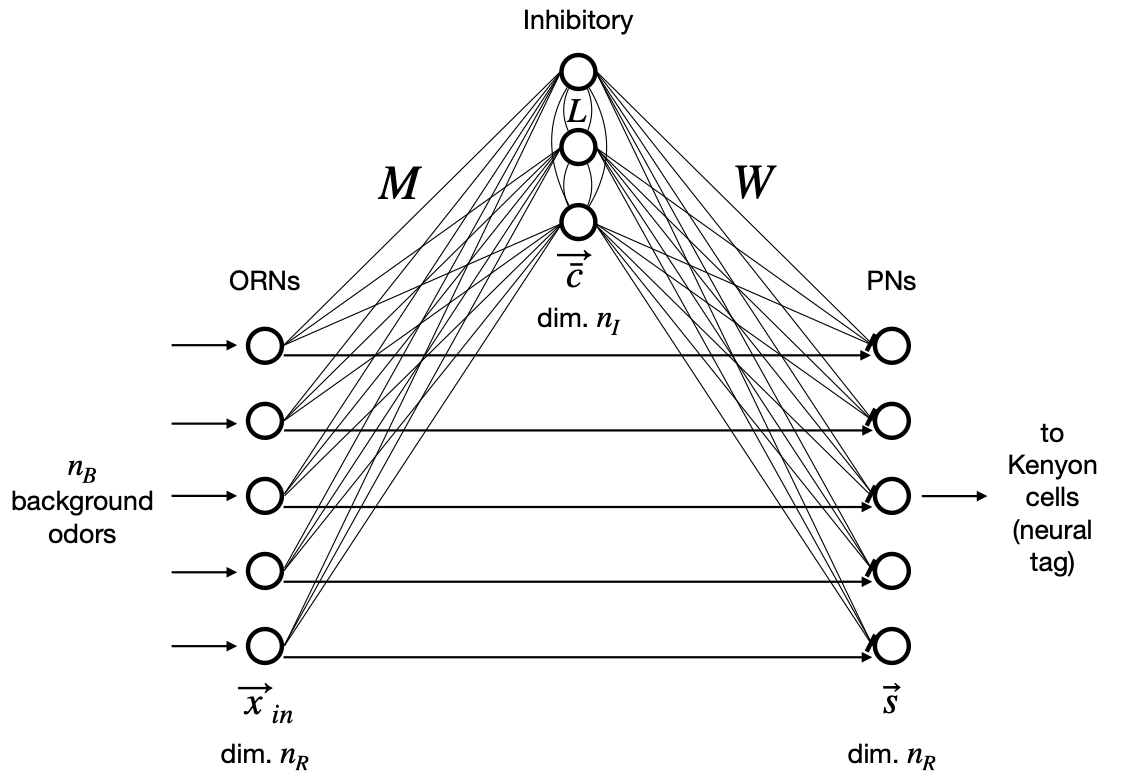
\includegraphics[width=0.8\textwidth]{figures/feedforward_inhibitory_network.pdf}
	\caption{Proposed olfactory habituation network model, where inhibitory neurons decompose the current background into components that are recombined to suppress the background ad its fluctuations. }
	\label{fig:inhibition_network}
\end{figure}

Second, the network has to learn inhibitory weights $W$ that can use the projections in the inhibitory neurons $\vec{\ovl{c}}$ to suppress the incoming background odor mixture. It turns out that local and Hebbian learning rules for the $W$ weights can be derived from a simple optimization problem, without regard to the details of how the projection weights $M$ and $L$ are learnt. We present these learning rules for $W$ synapses in this section; later on, they can be combined with IBCM neurons, PCA neurons, ICA neurons, or any other kind of inhibitory neurons. 

% Optimal W derivation. 
\subsection{Derivation of optimal inhibitory synaptic weights}
\label{subsect:optimal_inhib_weights}

% Cost function for W
\subsubsection{Cost function for $W$ optimization}
\label{subsubsect:cost_function}

During the learning phase (i.e. exposition to the background only), we want the inhibitory neurons to silence the activity of projection neurons in response to the varying input. Define $\vec{s}$ the vector of PN activities, with 

\beq
	\vec{s}= R(\vec{x}_{in} -  W\vec{\ovl{c}})   \quad ,
	\label{eq:pn_relu}
\eeq

where $R$ is an element-wise activation function (e.g., identity or ReLU), and $W\vec{\ovl{c}}$ is the output sent by the inhibitory neurons to projection neurons. Each column of $W$ is the vector $\vec{w}_j$ of synaptic weights leaving inhibitory neuron $j$ towards the different PNs in $\vec{s}$. 

We want the inhibitory weight matrix $W$ to minimize the norm of $\vec{s}$. This objective is encapsulated in the cost function

\beq
	C(W) = \frac12 \esper{\vec{s}^T \vec{s}} + \frac12 \frac{\beta}{\alpha} \esper{\vec{w}^T \vec{w}}
	\label{eq:cost_w}
\eeq

The first term ensures minimization of $\vec{s}$'s magnitude. The second term is a regularization ensuring $\vec{w}$ does not diverge when, for instance, $R$ is a ReLU function, such that large negative values of $\vec{w}$ would make $\vec{s}$ zero. In other words, the regularization ensures that the layer inhibits just enough the background and will still let through some of the new odor when it arrives. The parameter $\frac{\beta}{\alpha}$ controls the magnitude of this regularization (the choice of the form $\beta/\alpha$ will become clear below).

% Gradient calculation
\subsubsection{Gradient descent equations}
\label{subsubsect:gradient_descent}
We use gradient descent dynamics for the weights $\vec{w}_j$, 

\beq
	\frac{d \vec{w}_j}{dt} = - \alpha \vec{\nabla}_{\vec{w}_j} C(W)
	\label{eq:gradient_descent_w}
\eeq

so we need to compute the gradient of $C(W)$ with respect to each weight vector $\vec{w}_j$ (the $j$th column of $W$). The regularization term simply gives 
\beq
	\vec{\nabla}_{\vec{w}_j} \esper{\vec{w}^T \vec{w}} = 2 \esper{\vec{w}_j}   \,\,\, .
	\label{eq:gradient_regul}
\eeq
The $\vec{s}$ term gives 
\beq
	\vec{\nabla}_{\vec{w}_j} \esper{\vec{s}^T \vec{s}} = 2 \sum_k \esper{s^k \vec{\nabla}_{\vec{w}_j} s^k} \, \, \, .
	\label{eq:gradient_pn}
\eeq
We need to evaluate the derivative of $\vec{s} = R(\vec{x}_{in} - \sum_l \ovl{c}^l w^{kl})$, where $R$ is the PN activation function, for instance identity or ReLU. It is best worked out in index notation (Einstein summation of repeated indices applies except to $k$):

\begin{align}
	\vec{\nabla}_{\vec{w}_j} s^k & = \vec{\nabla}_{\vec{w}_j} R(x^k - w^k_l \ovl{c}^l w^{kl}) \nonumber \\
		&= - \hat{e}^i \frac{\partial}{\partial w^i_j} \left( w^k_l \ovl{c}^l \right) \frac{\partial R}{\partial s^k} \nonumber \\
		&= - R'(s^k) \hat{e}^i \delta_i^k \delta_l^j \ovl{c}^l \nonumber  \\
		&= -R'(s^k) \hat{e}^k \ovl{c}^j     \label{eq:gradient_calculation}
\end{align}

We will drop the averages and assume the rate $\alpha$ is small enough to effectively perform a time-averaging over the rapidly fluctuating inputs. We can finally combine equations \eqref{eq:gradient_regul}, \eqref{eq:gradient_pn}, and \eqref{eq:gradient_calculation} into equation \eqref{eq:gradient_descent_w} to obtain the optimal learning rule for the $\vec{w}_j$:

\beq
	\frac{d \vec{w}_j}{dt} = \alpha \ovl{c}^j \overrightarrow{sR'(s)} - \beta \vec{w}_j \quad ,
	\label{eq:learning_rule_w}
\eeq
where $\overrightarrow{s R'(s)}$ indicates that $R'$ is applied to $\vec{s}$ and multiplied to $\vec{s}$ element-wise. When $R$ is the identity function or a ReLu function, we can omit $R'(s)$: this is obvious for the identity case, while for the ReLU case, $s^k \underline{R'}(s^k) = s^k$, because $R'$ is the Heaviside step function ($1$ if $s^k > 0$, $0$ else) and $s^k$ in front of $R'$ is already zero anyways when $R'$ itself would be null. Note that $\alpha$ and $\beta$ are the learning rates of the $W$ synapses; usually, one takes $\beta < \alpha$ to ensure that $\vec{s}$ minimization is the dominant term of the cost function, and that background inhibition is efficient. 

The equation can be recast in matrix form for the whole $W$ using the outer product of $\vec{\ovl{c}}$ with $\vec{s}$ (we drop $R'$ for simplicity):

\beq
	\frac{dW}{dt} = \alpha {\vec{s}} \, \vec{\ovl{c}}^T - \beta W
	\label{eq:learning_rule_w_matrix}
\eeq

\subsection{Discussion of the inhibitory weights learning rule}
\label{subsect:discussion_w}

In component notation, equation \ref{eq:learning_rule_w} becomes
\beq
	\frac{d w^i_j}{dt} = \alpha \ovl{c}^j s^i R'(s^i) - \beta w^i_j \quad 
	\label{eq:learning_rule_w_components}
\eeq
This rule is seen to be completely local: $w^i_j$ only depends on the activities $\ovl{c}^i$ and $s^j$ of the neurons at its endpoints. It is also Hebbian, since the reinforcement of the connection is proportional to the product of those two activities. This makes such an inhibitory network biologically plausible. 

What exactly is being learnt with those weights $W$? The cost function introduced above aims, when $\beta = 0$, to minimize the norm of $\vec{s}$, that is (using $R = $ identity function for simplicity), to minimize $\| \vec{x} - W \vec{\ovl{c}} \|^2 = \| \vec{x} - W LM \vec{x}| \|^2$ with respect to $W$. For given $LM$ (learnt from IBCM, PCA, ICA, etc.), we know from linear algebra that the Moore-Penrose pseudo-inverse $(LM)^+$ minimizes this cost function{\protect
\footnote{Given a singular value decomposition (SVD) of a matrix $A = U \Sigma V^T$, the Moore-Penrose pseudo-inverse of $A$ is $A^+ = V \Sigma^+ U^T$, where $\Sigma^+$ has the inverse of the singular values on its diagonal. The pseudo-inverse solution to the minimization problem can actually be derived using SVD.}}. 
Therefore, the learning rule \eqref{eq:learning_rule_w} yields the Moore-Penrose pseudo-inverse -- or rather, an approximation of it, because of the regularization term. 


Therefore, the proposed network performs feedforward inhibition by learning approximately a projector on the background subspace, $P = \frac{\alpha}{\alpha + \beta}(LM)^+ (LM)$, and subtracting the input projection on that subspace from the full input: $\vec{s} = \vec{x} - P\vec{x}$. This leaves in $\vec{s}$ the input component that is orthogonal to the background (because of the regularization term, part of the orthogonal component persists in practice). In this sense, the network operates as an autoencoder with one hidden layer, learning a latent space to encode the olfactory background in the inhibitory neurons layer with matrices $LM$, and decoding them back to the full space with the weights $W$ to subtract that projection from the input, in $\vec{s} = \vec{x} - WLM \vec{x}$. 

The performance of this feedforward inhibition scheme will depend on the projections learnt via the $L$ and $M$ synaptic weights. We now discuss different models in the following sections, chiefly the IBCM model. 



\section{Presentation of the IBCM model of neuronal plasticity}
\label{sect:ibcm}

% Introduction to IBCM model alone. Goal: show how this model promises to learn more than the average. 
	% Equations, definitions
	% Intuition behind: competition between successive patterns. 
	% How it follows from a cost function favouring bimodal projections of data
	% Classical results: alternating backgrounds, specificity. Fluctuations of inputs are essential to converge to fixed points of the model, it needs to see statistics of the inputs. 
	% Network with mean field inhibition. Rewrite in terms of bar variables. "Parallel projection search"?
	% Oscillations

In 1982, Bienenstock, Cooper and Munro developed a model of synaptic plasticity -- subsequently called the BCM model after its authors -- to explain how neurons in the visual cortex become specifically responsive to certain visual patterns \cite{bienenstock_theory_1982}. The IBCM model, proposed 10 years later by Intrator and Cooper \cite{intrator_objective_1992}, modifies the threshold definition of the BCM model to have more robust dynamics. Moreover, Intrator and Cooper show that their modified model can be derived as a maximization problem of a cost function favouring the search of non-Gaussian projections of the input stimuli distribution. 
%The plasticity described by this model therefore drives neurons to form synapses that reinforce their response to some components of the visual stimulus and reduce their response to others. The hope is these properties of the model to components of fluctuating olfactory backgrounds. 

\subsection{Model equations}
\label{subsect:ibcm_equations}

\begin{figure}
	\centering
	\includegraphics[width=0.5\linewidth]{figures/cooper-bear2012_neuron_model.png}
	\caption{Description of a neuron in terms of its synaptic inputs $\vec{x}$ (denoted $\vec{d}$ on the figure) and weights $\vec{m}$and its activity $c$. Figure reproduced from \cite{cooper_bcm_2012}. }
	\label{fig:ibcm_neuron}
\end{figure}

An IBCM neuron is described by its $n_R$-dimensional synaptic weight vector $\vec{m}$ and its activity $c$, as depicted on figure~\ref{fig:ibcm_neuron}. The neuron receives input stimuli $\vec{x}(t)$, which can vary (quickly, randomly) over time, and its activity in response is the dot product of its weight vector and the input, $c(t) = \vec{m}(t) \cdot \vec{x}(t)$. The synaptic weights also evolve (slowly) over time in response to the stimuli and the IBCM neuron's own activity. 

The IBCM neuron's synaptic weights evolve according to \cite{intrator_objective_1992, udeigwe_emergent_2017}

\beq
	\frac{d \vec{m}}{d t} = \mu c \left(c - \Theta \right) \vec{x}
	\label{eq:ibcm_equation}
\eeq

where the threshold $\Theta$ tracks the recent average of the squared activity $c^2$:

\beq
	\frac{d \Theta}{dt} = \frac{1}{\tau_{\Theta}} (c^2 - \Theta)  
	\label{eq:ibcm_threshold}
\eeq

where we recall that $c(t) = \vec{m}(t) \cdot \vec{x}(t)$. 
The non-linear threshold evolves on a time scale $\tau_{\Theta}$ intermediate between the slow time scale of the synaptic weights learning, $\frac{1}{\mu}$, and the fast time scale of the input fluctuations, $\tau_b$. There are hence three time scales: $\tau_b \ll \tau_{\Theta} \ll  1 / \mu$, corresponding to the background process fluctuations, threshold averaging, and synaptic weights learning, respectively. The first condition ensures that the thresholds $\ovl{\Theta}^j$ properly average over the background distribution, while the latter ensures these thresholds reflect the average activity for the current $\vec{m}$, which can then evolve slowly in response. Undesirable oscillations of the synaptic weights occur if $\tau_{\Theta}$ and $1 / \mu$ are not different enough \cite{udeigwe_emergent_2017}. 

\subsection{Principles and properties of the model}
\label{subsect:ibcm_principles}

How does this model work? To begin with, notice that a quasi-static approximation on equation~\eqref{eq:ibcm_threshold} gives $\Theta = \esper{c^2} = \esper{(\vec{m} \cdot \vec{x})^2}$, where the synaptic vector $\vec{m}$ is approximately constant on the averaging time scale $\tau_\Theta$. The average is therefore mainly an average over the distribution of inputs $\vec{x}$. However, on a slow time scale, $\Theta$ evolves as the synaptic weights $\vec{m}$ change according to equation~\eqref{eq:ibcm_equation}. 

% Would probably need a simulation sample or some analytical calculation to support this claim and properly demonstrate this principle of the model. 
This change in the synaptic weights is driven by the rapid fluctuations of the input stimuli $\vec{x}$, in response to which the IBCM activity $c$ takes values above or below the average threshold $\Theta$. In the authors' words, ``whether synaptic strength increases or decreases depends upon the magnitude of the postsynaptic response as compared with a variable modification threshold.'' \cite{bienenstock_theory_1982}. In particular, as soon as the neuron starts to respond more to some stimuli than others, this nascent specificity is reinforced because those stimuli make the term $(c - \Theta)$ positive in eq.~\eqref{eq:ibcm_equation}, hence reinforcing the connections matching those inputs $\vec{x}$. Other stimuli cause below-average activation, hence $(c - \Theta)$ is negative and synaptic weights are suppressed in the direction of those hypostimulating $\vec{x}$. The threshold $\Theta$ evolves until the separation between specific and non-specific stimuli is maximized. Therefore, the IBCM neuron is driven to a specific state by the fast temporal competition between specific and non-specific stimuli causing reinforcement or depression of the synaptic weights, respectively. 


\subsection{IBCM fixed points for alternating inputs}
\label{subsect:ibcm_alternating}
The specificity property of the IBCM model is formalized by the following mathematical result, proved in the original article about the IBCM model \cite{intrator_objective_1992}. Let the input process $\vec{x}(t)$ be a random sequence of vectors in the set of linearly independent vectors $\{ \vec{x}_1, \vec{x}_2, \ldots, \vec{x}_{n_B} \}$, chosen independently at each time step with probabilities $\{p_k\}$. Then, the model has $n_B$ stable fixed points (degenerate if $n_B < n_R$)  for the synaptic weights $\vec{m}$, defined by null dot products with all but one of the input vectors, and a dot product $\vec{m} \cdot \vec{x}_k = 1/p_k$ with one of the $n_B$ input vectors; there is one stable fixed point for each input vector. In other words, in one of those fixed points, the IBCM neuron has zero response to all of the possible input components except one, call it $\vec{x}_k$, to which it responds specifically with amplitude $1/p_k$. 


\subsection{Cost function associated to the IBCM model}
\label{subsect:cost_function}

\begin{figure}
	\centering
	\includegraphics[width=0.5\linewidth]{figures/ibcm_loss_function_fixed_theta.pdf}
	\caption{In black: loss function minimized by the IBCM model equation, which is the gradient of the loss function with respect to $\vec{m}$. In grey: idealized distribution of the input stimuli projected on $\vec{m}$, that is, of the neuron's activity $c = \vec{m} \cdot \vec{x}$. The synaptic weights evolve to capture non-Gaussian (scalar) projections of the input (vector) distribution. }
	\label{fig:loss_function}
\end{figure}

The specificity property of IBCM  neurons can also be understood in the light of the objective function minimized by  equation~\eqref{eq:ibcm_equation} derives. This loss function is designed to find synaptic weights $\vec{m}$ on which the projection of the distribution of stimuli $\vec{x}$ is non-Gaussian or even multimodal. Hence, it involves higher moments of the distribution of neuron activities: 

\beq
	L_{m}(c, \Theta) = -\mu \left(\frac13 c^3 - \frac14 \Theta c^2 \right)   \quad \mathrm{where \, we \, set} \, \Theta = \esper{c^2}
	\label{eq:loss_function}
\eeq

Taking the gradient of this loss function, illustrated in figure \ref{fig:loss_function}, with respect to $\vec{m}$ and setting it equal to $\frac{d\vec{m}}{dt}$ yields equation \eqref{eq:ibcm_equation}. This loss function goes to $-\infty$ for large $c$, so it looks like it has no minimum, but one must recall that the threshold $\Theta$, and hence the barrier at $c=\Theta/2$, moves with the average $c$. The successive stimuli must cause activation levels $c$ that fluctuate from one side to the other of $\Theta/2$. The only way to minimize the average cost function is to have most stimuli landing on the local minimum, at $c=0$, and a few landing to the right of $c > 3\Theta/4$, where the loss function takes large negative values: these are the non-specific and the specific stimuli, respectively. When $\vec{m}$ is at steady-state and the threshold $\Theta$ is constant, the distribution of values of $c$ tends to have one mode at $c=0$ and another at $c > 3\Theta/4$, as illustrated on figure \ref{fig:loss_function}. 



% Presentation of the proposed inhibition network when IBCM neurons are used in it
\section{Olfactory inhibition network with IBCM neurons}
\label{sect:ibcm_inhibition}
Now that we have defined a generic learning rule for the $W$ inhibitory weights (section \ref{sect:inhib_network}) and introduced the IBCM model (section \ref{sect:ibcm}) of neuronal specificity, we can show how that model can be used for the neurons in the inhibitory layer of the feedforward inhibition network of figure \ref{fig:inhibition_network}. The intuition is that IBCM neurons slowly become specific (through $M$) to odor components of the olfactory background and suppress them via the $W$ synapses, while new odors are not suppressed because no IBCM neuron has become specific to them yet. We will also give details on how this network's learning process can be numerically simulated for various stochastic input processes $\vec{x}_b(t)$ representing the olfactory background. 

Table \ref{tab:symbols} summarizes the notation used thus far and introduced below. 

\begin{table}[p]
\centering
\input{tables/olfaction_table_symbols.tex}
\caption{Definition of notation in this model: abbreviations, variables, parameters and time scales. }
\label{tab:symbols}
\end{table}


\subsection{Nonlinear response function}
\label{subsect:nonlinear_neuron}
For large simulations, the IBCM model is more stable numerically if we apply a nonlinear saturating function to the activity $c$ of the neuron. Specifically, we choose a tanh function with a high threshold for saturation. Thus, the activity of a neuron in response to stimulus $\vec{x}$ becomes
\beq
c = \sigma(\vec{m} \cdot \vec{x}) = c_{\mathrm{sat}} \tanh{\left( \frac{\vec{m} \cdot \vec{x}}{c_{\mathrm{sat}}}\right)}
\label{eq:nonlinear_neuron}
\eeq

We make $c_{\mathrm{sat}}$ quite large, typically $c_{\mathrm{sat}} \approx 50$. Thus, for small neuron responses $\vec{m} \cdot \vec{x}$, the tanh function is in the linear regime, $c \approx \vec{m} \cdot \vec{x}$, such that most analytical calculations assuming a linear response still hold true; the nonlinearity only prevents very large neuron responses which otherwise would cause divergences in numerical simulations with strong fluctuations. 

The dynamical equations get modified accordingly. By taking the gradient of the cost function introduced above, with $c$ including the tanh activation function, the time derivative of $\vec{m}$ becomes (with $\frac{d \tanh(u)}{du} = 1 - \tanh^2(u)$)

\beq
	\frac{d \vec{m}}{d t} = \mu c \left(c - \Theta \right) \vec{x} \sigma'(\vec{x} \cdot \vec{m}) = \mu c \left(c - \Theta \right) \vec{x} (1 - c^2) \,\,.
	\label{eq:ibcm_equation_nonlinear}
\eeq



\subsection{Network of IBCM neurons with feedforward coupling}
\label{subsect:ibcm_network}

We now imagine a network of $n_I$ IBCM neurons, each connected to the $n_R$ input nodes and weakly coupled to the other IBCM neurons. 
% Idea: have different neurons connected to subparts of the inputs. So each neuron sees different components, maybe that is more efficient? Could help convergence speed a lot, but might lose some inhibition ability. But not if number of components much smaller than number of dimensions; actually the number of connections per IBCM neurons would set the max number of components the network can learn to inhibit (e.g. if each IBCM is connected to 6 input nodes, that's n_R=6 dimensions per IBCM, so at most specific to one of six components). 
% Is that dividing and conquering the problem, or would it fail equally/more than fully connected case? 
They can repress each other such that the activity of the $j$th neuron after inhibition is

\beq
	\ovl{c}^j = c^j - \eta \sum_{k \neq j} c^k = c^j(1 + \eta) -  \eta \sum_k c^k 
	\label{eq:inhibited_activity}
\eeq

%(
where $\eta$ is a coupling parameter $\in [0, 1)$ %]
and $c^k = \vec{m}^k \cdot \vec{x}$ is the activity of neuron $k$ before coupling is applied. Equation \eqref{eq:inhibited_activity} corresponds to a lateral connection matrix $L$ that has $1$ on its diagonal and $-\eta$ elsewhere. 
Such lateral weights can also be derived as a mean-field approximation for other choices of $L$. If we let $\vec{m}^k$ be the $k$th \emph{row} of the matrix $M$ ($n_I \times n_R$), then equation \eqref{eq:inhibited_activity} can simply be written in matrix form as 

\beq
	\vec{\ovl{c}}= L M \vec{x}
	\label{eq:inhibited_activity_matrix}
\eeq
which matches the inhibitory layer of the network structure presented in figure \ref{fig:inhibition_network}. 

In turn, the appropriate thresholds for neurons, which we call $\ovl{\Theta}^j$, are based on the inhibited activities $\ovl{c}^j$:

\beq
	\frac{d \ovl{\Theta}^j}{dt} = \frac{1}{\tau_{\Theta}} ((\ovl{c}^j)^2 - \ovl{\Theta}^j)
	\label{eq:inhibited_theta}
\eeq

To derive proper dynamical equations for the learning of $\vec{m}^k$ (rows of $M$) in the inhibition network with IBCM neurons, we start from the total cost function $L^{tot}_m(\{\ovl{c}^j\})$, which is the sum of single-neuron costs with $\ovl{c}^k$ replacing $c^k$:

\beq
	L^{tot}_m(\{\ovl{c}^j\}) = -\mu \sum_j  \left(\frac13 (\ovl{c}^j)^3 - \frac14 \ovl{\Theta}^j (\ovl{c}^j)^2 \right)
	\label{eq:inhibited_cost}
\eeq

Taking the gradient of $L_m$ with respect to $\vec{m}^j$ gives rise to two terms, because each $\ovl{c}^k$, $k \neq j$, also depends on $\vec{m}^j$ in the $-\eta \sum_{l\neq k} \ovl{c}^k$ part. The proper dynamical equations are then

\beq
	\frac{d \vec{m}^j}{dt} = \mu \left[ \ovl{c}^j(\ovl{c}^j - \ovl{\Theta}^j) - \eta \sum_{k \neq j} \ovl{c}^k (\ovl{c}^k - \ovl{\Theta}^k )  \right] \vec{x}
	\label{eq:ibcm_equation_coupled}
\eeq


The feedforward coupling through $L$ has been reported to favor steady-states where different neurons are specific to different input components \cite{castellani_solutions_1999}. Presumably, it enlarges the basins of attraction of those network steady-states, but this is hard to show numerically or analytically (because the complete phase space is $n_I \times n_R$-dimensional). 


\subsection{General rules to find IBCM fixed points analytically}
\label{subsect:general_fixed_points}
The fixed points of the IBCM equations are important to understand, because they tell what projections will be learnt by the inhibitory neurons. 

We say an IBCM neuron in the network has reached a fixed point when its input synaptic weights $\vec{m}$ are stationary, i.e. \emph{on average} constant over time; fluctuations in $\vec{x}(t)$ mean that $\vec{m}(t)$ will also be stochastic. From equation \eqref{eq:ibcm_equation_coupled}, 

\beq
	\frac{d \esper{\vec{m}^j}}{dt} = 0 = \esper{\ovl{c}^j(\ovl{c}^j - \ovl{\Theta}^j)}  - \eta \sum_{k \neq j} \esper{\ovl{c}^k(\ovl{c}^k - \ovl{\Theta}^k)} \quad \forall j
	\label{eq:ibcm_general_steady}
\eeq

Defining terms $A^j = \esper{\ovl{c}^j(\ovl{c}^j - \ovl{\Theta}^j)}$, this system of equations can be put in matrix form, 
\beq
	L A = 0
	\label{eq:ibcm_general_steady_matrix}
\eeq
where $A$ is the $n_I$-dimensional vector of the $A^j$ just defined and $L$ is the $n_I \times n_I$ matrix of lateral connection weights with $1$ on the diagonal and $-\eta$ everywhere else. $L$ is a circulant matrix: each row is a cyclic permutation of the previous row by one element to the right. Its eigenvectors and eigenvalues have an analytic form, from which we can compute the determinant and tell whether $L$ is invertible{\protect
\footnote{See Wikipedia page \url{https://en.wikipedia.org/wiki/Circulant_matrix} and Scipy's function to solve circulant systems of equations \url{https://docs.scipy.org/doc/scipy/reference/generated/scipy.linalg.solve_circulant.html} 
}}. It turns out that $L$'s eigenvalues are $1 - (n_I-1)\eta$ (once) and $\eta + 1$ (degenerate $n_I-1$ times). Hence, unless we are in the pathological cases $\eta = -1$ or $\eta = \frac{1}{n_I-1}$, $L$ is invertible and the unique solution is $A = L^{-1} 0 = 0$. Therefore, in general, the fixed points of the IBCM network are found by setting each term to zero individually:
\beq
	\esper{\ovl{c}^j(\ovl{c}^j - \ovl{\Theta}^j)} = 0 \quad \forall j \in \{1, 2, \ldots, M\}
	\label{eq:ibcm_fixed_points}
\eeq

Then, defining new ``reduced'' synaptic weights

\beq
	\vec{\ovl{m}}^j = \vec{m}^j - \eta \sum_{k \neq j} \vec{m}^k 
	\label{eq:reduced_synaptic_weights}
\eeq

such that $\ovl{c}^j = \vec{\ovl{m}}^j \cdot \vec{x}$ allows one to decouple the steady-state equations \eqref{eq:ibcm_fixed_points} by solving in terms of the $\vec{\ovl{m}}^j$. In terms of those reduced variables, the problem of finding fixed points for the IBCM network with feedforward inhibition reduces to finding the fixed points for a single IBCM neuron. 
%Network fixed points are just all possible combinations of single-neuron fixed points, combined independently (if one neuron has $S$ stable fixed points, there are $S^M$ possible combinations). 

%% TODO: show a bit more how to develop this equation, inserting the dot product, etc? Maybe not relevant, depends too much on x(t)? But we can at least mention some approximations on neglecting correlations, no?


% Recovering the synaptic weight vectors \vec{m} from the \vec{\ovl{m}}
Afterwards, the actual synaptic weights $\vec{m}^j$ can be found from the $\vec{\ovl{m}}^j$ solutions by inverting the matrix equation
\beq
	\ovl{M} = L M
\eeq

where $M$ and $\ovl{M}$ are $n_I \times n_R$ matrices where each row is a vector $\vec{m}^j$ or $\vec{\ovl{m}}^j$ and $L$ is the circulant matrix of lateral weights. This matrix, applied to the input $\vec{x}$, directly gives the projections computed by the inhibitory neurons in the network of figure \ref{fig:inhibition_network}, $\vec{\ovl{c}} = LM \vec{c} = \ovl{M} \vec{x}$. 

From the eigenvectors and eigenvalues of $L$, one can compute that elements of $L^{-1}$ are 
\beq
	L^{-1}_{ij} = \left\{ 
		\begin{array}{ll}
			\frac{(n_I-2)\eta - 1}{(n_I-1)\eta^2 + (n_I-2) \eta - 1} 	& \text{on the diagonal} \\
			\frac{-\eta}{(n_I-1)\eta^2 + (n_I-2) \eta - 1}			& \text{off-diagonal} \\
		\end{array}
	\right.
	\label{eq:inverse_circulant_elements}
\eeq

Hence, the synaptic weights $M$ can be recovered from the reduced ones, if necessary, as

\beq
	\vec{m}^j = \frac{[(n_I-2) \eta - 1] \vec{\ovl{m}}^j - \eta \sum_{k \neq j} \vec{\ovl{m}}^k}{(n_I-1)\eta^2 + (n_I-2) \eta - 1}  \quad \mathrm{if} \, \eta \neq \frac{1}{n_I-1} \,\,\mathrm{or}\,\, -1 \,\, .
	\label{eq:inverse_circulant_mvecs}
\eeq

There is no need to invert $L$ when using this network of IBCM neurons to inhibit a fluctuating background; $\ovl{M} = LM$ is the relevant projection matrix to apply to inputs. But it may be useful to compute $M$ from $\ovl{M}$ when comparing analytical predictions to simulations. 

%The eigenvalues of $L$ are $1 - (n_I-1)\eta$ and $n_I-1$ times $\eta + 1$, so if $\eta = \frac{1}{n_I-1}$, there are zero eigenvalues and the matrix is not invertible; this is the pathological case for fixed points already noted above. 



\subsection{IBCM habituation network equations}
\label{subsect:network_equations}

Here, we summarize the network equations when inhibitory neurons evolve according to the IBCM model. 

First, in a linear approximation (to be improved in future work with better models of ORN activation), the input process at the ORN layer, $\vec{x}_b(t)$, will generally be a mixture of odor vectors $\vec{x}_{\gamma}$ present simultaneously at varying concentrations:
\beq
	\vec{x}_b(t) = \sum_{\gamma} \nu_{\gamma}(t) \vec{x}_{\gamma}
	\label{eq:background_mixture}
\eeq
during the background learning phase. When a new odor $\vec{x}_n$ is introduced at some time $T$, the input will then be a mixture $\vec{x}(T) = \vec{x}_b(T) + f \vec{x}_n$, where $f$ controls the concentration of that odor compared to the background. This is different from the alternating stimuli usually studied in the IBCM literature (section \ref{subsect:ibcm_alternating}). Increasingly complex input processes will be described and analyzed in the following sections. Generally speaking, the background $\vec{x}(t)$ will fluctuate with a fast correlation time scale $\tau_b$. 

The IBCM neurons receive the input process $\vec{x}(t)$ from the ORN layer and evolve according to the IBCM network equations with constant feedforward coupling $L$ as stated in section \ref{subsect:ibcm_network}:

\begin{align*}
	\frac{d \vec{m}^j}{dt} &= \mu \left[ \ovl{c}^j (\ovl{c}^j - \ovl{\Theta}^j) - \eta \sum_{k \neq j} \ovl{c}^k (\ovl{c}^k - \ovl{\Theta}^k )  \right] \vec{x}(t) 			\tag{\ref{eq:ibcm_equation_coupled}} \\
	\frac{d \ovl{\Theta}^j}{dt} &= \frac{1}{\tau_{\Theta}} ((\ovl{c}^j)^2 - \ovl{\Theta}^j)  \tag{\ref{eq:inhibited_theta}}  \\
	\vec{\ovl{c}}(t) &= L M \vec{x}(t)		\tag{\ref{eq:inhibited_activity_matrix}}
\end{align*}

with $L$ having $1$ on the diagonal and $-\eta$ off-diagonal and $\vec{m}^j$ being the $j$th row of $M$. 

Then, the inhibitory weights $W$ evolve to minimize the activity of projection neurons, $\vec{s}$, during exposition to the olfactory background, as derived in section \ref{subsect:optimal_inhib_weights}:

\begin{align*}
	\frac{d \vec{w}_j}{dt} &= \alpha \ovl{c}^j \vec{s} - \beta \vec{w}_j  	\tag{\ref{eq:learning_rule_w}} \\
	\vec{s} &= R(\vec{x}_{in} -  W\vec{\ovl{c}})   \tag{\ref{eq:pn_relu}}
\end{align*}
where $R$ is either the identity or the ReLU function, so $R'$ could be omitted from \eqref{eq:learning_rule_w}. 

The inhibition vector $W \vec{\ovl{c}} = WLM\vec{x}(t)$ is subtracted from $\vec{x}(t)$, at any time $t$. Once the $\vec{m}^j$ and $\vec{w}_j$ have reached their steady-state, fluctuations of the background should be continually suppressed as they come, since $WLM\vec{x}(t)$ instantaneously track variations of $\vec{x}(t)$ in the olfactory background subspace, on the fast time scale $\tau_b$. The exact configuration of $W$ that optimizes inhibition will depend strongly on the input process and the $\vec{m}^j$ learnt, but the general idea is that each IBCM neuron will become specific to one odor in the background (e.g. for an alternating background), so the associated $\vec{w}_j$ will learn an image of that odor and subtract it when the IBCM neuron fires (i.e. detects the presence of that odor). 

\subsection{Simulation details}  % Will give some intuition about how the system works, the different time scales combined, etc. 
\label{subsect:network_simulation}
There are four well separated time scales in this inhibitory network model: $\tau_b \ll \tau_\Theta \ll 1/\mu \leq 1/\alpha$. We need to run simulations with small time steps on the order of $\tau_b$ at most, because the thresholds $\Theta$ need to ``see'' multiple values of the background process to perform proper averaging, and the synaptic weight vectors $\vec{m}$ need to ``see'' temporal competition between different background vectors to become specific. We set the time step $\Delta t = 1$ and define other time scales relative to this unit. The number of neurons $n_I$ should be the expected number of background odor components $n_B$, to ensure that each component can be learnt and inhibited. We use weak feedforward coupling $\eta$ between IBCM neurons, because strong coupling blocks the network near the origin and delays habituation too long. Table \ref{tab:parameter_values} lists typical parameter values used in simulations. 
	% Note: could use some tau-leaping algorithm to update m only once in a while? Or at least update theta only once in a while. Unclear how to update m only once in a while because need temporal competition between patterns. Maybe take one every tau_b and make a larger dt so the impact of each is more significant? 

\begin{table}
	\centering
	\input{tables/typical_ibcm_parameter_values.tex}
	\caption{Typical parameter values for simulation of the IBCM inhibition network. Some dimensions ($n_R$, $n_B$) and other parameters depend on the choice of background process. }
	\label{tab:parameter_values}
\end{table}

The model equations are solved using a simple Euler scheme with step size $\Delta t$. At every step, variables are updated to $t+\Delta t$ based on their derivatives evaluated at time $t$. Therefore, when only the current value of a variable is recorded (to avoid memory issues), one must be careful to update some variable $A$ only after all other variables depending on it have been updated. Otherwise, incorrect time correlations are introduced. For our inhibition network, variables can be updated in the following order (decreasing order of dependency):
\begin{enumerate}
	\item Update the inhibition weights $\vec{w}_j$ to $t+\Delta t$ based on equation \eqref{eq:learning_rule_w}, using the projection neurons activity $\vec{s}(t)$ and the IBCM neurons' activities $\ovl{c}^j(t)$ available from the previous iteration. 
	\item Update the IBCM synaptic weights $\vec{m}^j$ based on equation \eqref{eq:ibcm_equation_coupled}, using $\ovl{c}^j(t)$ and $\ovl{\Theta}^j(t)$ from the previous iteration.
	\item Update the IBCM thresholds $\ovl{\Theta}^j$ with equation \eqref{eq:inhibited_theta} using the $\ovl{c}^j(t)$ from the previous iteration. 
	\item Update the input process to $\vec{x}(t + \Delta t)$. 
	\item Evaluate the activity of IBCM neurons $\vec{\ovl{c}}(t + \Delta t)$ in response to $\vec{x}(t+\Delta t)$ with $\vec{m}^j(t+\Delta t)$ and the constant coupling $L$ as in equation \eqref{eq:inhibited_activity}.  	
	\item Apply inhibition on the PN neurons layer by evaluating equation \eqref{eq:pn_relu} with $\vec{w}_j(t+\Delta t)$ and $\ovl{c}^j(t+\Delta t)$. 
\end{enumerate}





%%% Solution of IBCM equations for simple examples
\section{IBCM network solution for simple backgrounds}
\label{sect:ibcm_simple_examples}
% IBCM network on a 2-odor toy model. As a proof of principle that this network has the desired properties. 
\subsection{Toy example: two-odor Gaussian background}
\label{subsect:2d_model}

% Inhibitory part solution
% Analytics, numerics. 
% New odor recognition? Meh, drop it, we are in 2d case anyways. 
% Notice that if d > n_odors, d-n dimensions not specified. Is that a problem? Not sure, we will see. 

% Background process, Ornstein-Uhlenbeck, simulation method. 
\subsubsection{Background process}
\label{subsubsect:2d_background}
We first consider a toy version of an olfactory background, which is a linear combination of two odors with fluctuating proportions. Let the input be

\beq
	\vec{x}(t) = \left(\frac12 + \ovl{\nu}(t)\right) \vec{x}_a + \left(\frac12 - \ovl{\nu}(t)\right) \vec{x}_b
	\label{eq:2d_mixture_process}
\eeq

where $\vec{x}_a$ and $\vec{x}_b$ are constant $n_R$-dimensional vectors and $\ovl{\nu}(t)$ follows the Ornstein-Uhlenbeck process

\beq
	\frac{d \ovl{\nu}}{dt} = -\frac{1}{\tau_b} \ovl{\nu} + \sqrt{\frac{2 \sigma^2}{\tau_b}} \xi(t)
	\label{eq:oh_process_1d}
\eeq

where $\xi(t)$ is white noise, $\tau_b$ is the autocorrelation time scale, and the steady-state distribution of $\ovl{\nu}$ is a zero-mean, $\sigma^2$ variance normal distribution. We typically choose $\sigma^2 = 0.09$ ($\sigma = 0.3$), so fluctuations of $\frac12 \pm \ovl{\nu}$ past $0$ or $1$ are infrequent but possible. 

To simulate the Ornstein-Uhlenbeck (O-U) process $\ovl{\nu}(t)$ numerically, we use an exact update rule for finite time steps $\Delta t$ derived from the analytical solution of the O-U process, taking the last time step as a new deterministic initial condition~\cite[eq.~2.47]{gillespie_mathematics_1996}:

\beq
	\ovl{\nu}(t + \Delta t) = \ovl{\nu}(t) e^{-\Delta t / \tau_b} + \sqrt{\sigma^2 \left(1 - e^{-2 \Delta t / \tau_b}  \right)}\, \xi(t)
	\label{eq:exact_update_rule_o-u}
\eeq

where $\xi(t)$ is white noise. The coefficients of $\ovl{\nu}(t)$ and $\xi(t)$ can be computed in advance. This rule ensures a steady-state distribution of $\ovl{\nu}$ with the desired variance $\sigma^2$ even though the simulation time step is on the order of $\tau_b$. 


% IBCM part solution
\subsubsection{Analytical results: IBCM fixed points}
\label{subsubsect:2d_model_analytical}

To understand analytically how this binary mixture background can be inhibited by the proposed network, we start by calculating the steady-state of the IBCM neurons' $\vec{m}^j$ synaptic weights; the inhibitory weights $W$ follow from them. The fixed points equations to solve for the IBCM neurons are, from equation \eqref{eq:ibcm_fixed_points}, 

\beq
	0 = \esper{\{ \vec{\ovl{m}}^j \cdot \vec{x}(t) \}^2 \vec{x}(t)} - \esper{\{ \vec{\ovl{m}}^j \cdot \vec{x}(t) \} \ovl{\Theta}^j \vec{x}(t)} \quad \forall j \in \{1, 2, \ldots, n_I \} \, \, .
	\label{eq:ibcm_fixed_points_developed}
\eeq

Since those $M$ equations are identical, we can drop the $j$ indices and concentrate on one of them. Some approximations are necessary to make analytical progress. 
The first approximation we make is to replace $\ovl{\Theta} = \esper{\ovl{c}^2}$, that is, we neglect correlations between $\Theta$ and $\ovl{\nu}$ or $\vec{m}$. 
The second approximation is that correlations between $\vec{\ovl{m}}^j$ and $\ovl{\nu}(t)$ are negligible; this is fair if time scales $1/\mu$, $\tau_{\Theta}$ and $\tau_b$ are well separated. Third, we assume the variance of $\vec{\ovl{m}}^j$ will be small, since variations in $\vec{\ovl{m}}$ would come from rapid changes in $\ovl{\nu}(t)$ and ensuing fluctuations in $\ovl{\Theta}$. Hence, we can treat $\vec{\ovl{m}} = \esper{\vec{\ovl{m}}}$ as constant in the equation. 

Moreover, we rewrite $\vec{x}(t) = \vec{x}_d + \ovl{\nu}(t) \vec{x}_s$, where $\vec{x}_d = \frac12 (\vec{x}_a + \vec{x}_b)$ (deterministic part) and $\vec{x}_s = \vec{x}_a - \vec{x}_b$ (stochastic part). From these new vectors appear the dot products $\ovl{c}_d = \esper{\vec{\ovl{m}}} \cdot \vec{x}_d$ and $\ovl{c}_s = \esper{\vec{\ovl{m}}} \cdot \vec{x}_s$, such that $\ovl{c} = \ovl{c}_d + \ovl{\nu}(t) \ovl{c}_s$. We can solve for the two dot products $\ovl{c}_d$ and $\ovl{c}_s$ because they specify the fixed points completely when there are $K=2$ background components. In light of our approximations, they are constant with respect to the average operator in equation \eqref{eq:ibcm_fixed_points_developed}, which becomes

\begin{align}
	0 &= \esper{(\ovl{c}_d + \ovl{\nu} \ovl{c}_s)^2 (\vec{x}_d + \ovl{\nu} \vec{x}_s)} - \esper{(\ovl{c}_d + \ovl{\nu} \ovl{c}_s)^2}\esper{(\ovl{c}_d + \ovl{\nu} \ovl{c}_s) (\vec{x}_d + \ovl{\nu} \vec{x}_s)}  \nonumber \\
	0 &= (\ovl{c}_d^2 + \sigma^2 \ovl{c}_s^2 - \ovl{c}_d^3 - \ovl{c}_d \ovl{c}_s^2 \sigma^2) \vec{x}_d + (2 \ovl{c}_s \ovl{c}_d - \ovl{c}_d^2 \ovl{c}_s -\sigma^2 \ovl{c}_s^3)\sigma^2 \vec{x}_s  \label{eq:fixed_points_2d_developed}
\end{align}

Since $\vec{x}_d$ and $\vec{x}_s$ are linearly independent, both coefficients must be zero, leading to a system of two nonlinear equations for $\ovl{c}_d$ and $\ovl{c}_s$:

\begin{align}
	0 &= \ovl{c}_d^3 - \ovl{c}_d^2 - \sigma^2 \ovl{c}_s^2 + \ovl{c}_d \ovl{c}_s^2 \sigma^2 \\
	0 &= \sigma^2 \ovl{c}_s ( \ovl{c}_d^2 + \sigma^2 \ovl{c}_s^2 - 2\ovl{c}_d)
\end{align}

From these two equations, we find the following solutions{\protect \footnote{
There is also a solution $s=d=0$ corresponding to $\vec{m} = 0$, which is unstable.
}}:

\beq
	\ovl{c}_d =  \vec{\ovl{m}} \cdot \vec{x}_d = 1 \,\, \mathrm{and} \,\, \ovl{c}_s = \vec{\ovl{m}} \cdot \vec{x}_s = \pm \frac{1}{\sigma}
	\label{eq:ibcm_2d_solution_sd}
\eeq

or, in terms of the dot products with $\vec{x}_a$ and $\vec{x}_b$:

\beq
	\vec{\ovl{m}}^{\pm} \cdot \vec{x}_a = 1 \pm \frac{1}{2 \sigma}  \,\, \mathrm{and} \,\, 1 \mp \frac{1}{2 \sigma}
	\label{eq:ibcm_2d_solution_ab}
\eeq

From the two dot products, we can build $\vec{\ovl{m}}$ and then $\vec{m}$ from equation \eqref{eq:inverse_circulant_mvecs}. 
Hence, we find two different stable fixed points, which we call $\vec{\ovl{m}}^+$ and $\vec{\ovl{m}}^-$ to indicate which sign the dot product with $\vec{x}_s$ takes. To understand better what these fixed points imply, let's compute the response of an IBCM neuron at either fixed point to some stimulus $\vec{x}(t)$:

\beq
	\ovl{c}^{\pm} = \vec{\ovl{m}}^{\pm} \cdot (\vec{x}_s + \ovl{\nu}(t) \vec{x}_d) = 1 \pm \frac{\ovl{\nu}}{\sigma}
	\label{eq:ibcm_2d_response}
\eeq

We notice that $\ovl{c} = 0$ when $\ovl{\nu} = \mp \sigma$, that is, \emph{the IBCM neuron is non-responsive to an odor component one standard deviation away on one side of the average background, while it responds strongly to odors on the other side of the average}. Thus, the model's specificity property, well-studied for alternating backgrounds, is preserved for inputs with continuous variations, now with vectors one standard deviation away from the average representing the different components that can be ``selected'' by the IBCM neuron. In other words, the neuron becomes selective for $\vec{x}(\ovl{\nu} = \pm \sigma)$. 

%Since there are $K = 2$ linearly independent vectors in the background, we can use $n_R=2$ dimensions: the effective space of $\vec{m}$ vectors is the same vector space as $\vec{x}$, since $\frac{d\vec{m}}{dt} \propto \vec{x}(t)$. If the neurons have in reality more synapses, we can redefine coordinates to have 2 dimensions. The remaining $n_R-2$ dimensions of $\vec{m}$ stay constant over time and are determined by the initial conditions. 
% The part of $\vec{m}$ in the orthogonal complement of this vector space remains constant over time and is determined by the initial conditions. 
%In general, with a $n_B$-dimensional vector space of $\vec{x}$, each fixed point is in reality a $(n_R-n_B)$-dimensional manifold of fixed points. 

\subsubsection{Analytical results: convergence time}
\label{subsubsect:convergence_time_2d}
For our habituation model to be realistic, it must converge reasonably fast to a steady-state. The convergence time of a single IBCM neuron can be estimated analytically at least in the two-odor toy model; this analysis reveals the main parameters influencing how long it takes to habituate to a fluctuating background (assuming the convergence of inhibitory weights $W$ occurs at a similar pace, which is the case numerically)\protect{\footnote{
The following calculation was devised by Gautam Reddy. 
}}.

To begin with, we make a quasi-static approximation on the threshold $\Theta$, assuming it averages over the fast background fluctuations but also converges fast enough to track the slow variations of $\vec{m}$:
\begin{equation*}
	\Theta \approx \mathbb{E}_{\ovl{\nu}}\left[c^2\right] = \mathbb{E}_{\ovl{\nu}}\left[(\vec{m} \cdot \vec{x}_d + \ovl{\nu} \vec{m} \cdot \vec{x}_s)^2\right] = c_d^2 + \sigma^2 c_s^2
\end{equation*}
where we made use of $\esper{\ovl{\nu}} = 0$ and we have defined variables $c_d = \vec{m} \cdot \vec{x}_d$ and $c_s = \vec{m} \cdot \vec{x}_s$ for the dot products of $\vec{m}(t)$ with the constant vectors $\vec{x}_d = \frac12 \vec{x}_a + \frac12 \vec{x}_b$ and $\vec{x}_s = \vec{x}_a - \vec{x}_b$. Then, the trick is to derive dynamical equations (on the $\mu$ time scale) for those variables by taking the dot product of $\frac{d \vec{m}}{dt}$ with $\vec{x}_s$ and $\vec{x}_a$, averaging over fast time scales of $\ovl{\nu}(t)$, and using the quasi-static $\Theta$ above. For $c_s$ for instance, we calculate (using $c = c_d + \ovl{\nu} c_s$ and the orthogonality of $\vec{x}_d$ and $\vec{x}_s$ that holds when $\vec{x}_a$ and $\vec{x}_b$ have an equal norm)

\begin{align}
	\frac{d c_d}{dt} &= \esper{ \frac{d \vec{m}}{dt} \cdot \vec{x}_d} = \mu \esper{(c_d + \ovl{\nu} c_s)(c_d + \ovl{\nu} c_s - \Theta)} x_d^2  \nonumber \\
	&= \mu \left(c_d^2 + \sigma^2 c_s^2 - c_d \left(c_d^2 + \sigma^2 c_s^2 \right) \right) x_d^2 \nonumber \\
	&= \mu x_d^2 (1 - c_d)\left(c_d^2 + \sigma^2 c_s^2 \right) \,\,\, .
	\label{eq:c_d_dynamics}
\end{align}

By a similar calculation, we find for $c_s$

\beq
	\frac{d c_s}{dt} = \mu \sigma^2 x_s^2 c_s \left(2 c_d - \left(c_d^2 + \sigma^2 c_s^2 \right) \right) \,\,\, .
	\label{eq:c_s_dynamics}
\eeq

% TODO: finish typesetting analysis in March15 entry, two phases, etc. See also correction made on August 15. 
From equations \eqref{eq:c_d_dynamics} and \eqref{eq:c_s_dynamics}, we can conclude there will be two phases to the dynamics if the initial values of $c_s(0) = \epsilon_s$ and $c_d(0) = \epsilon_s$ are small, and $\sigma^2$ is small also. The only positive term in $\frac{d c_s}{dt}$ contains $c_d$; hence, as long as $c_d$ is small, $c_s$ will remain close to zero. The first phase therefore consists in the growth of $c_d$ to its steady-state value of $1$, while $c_s$ remains approximately equal to its initial value, $\epsilon_s$. We call $t_d$ its duration. After $c_d$ has converged, the second phase consists in the growth of $c_s$. We call $t_s$ the duration of that phase. Hence, $c_s$ reaches steady-state after a total time of $t_d + t_s$. 

We compute $t_d$ (first phase duration) by integrating equation \eqref{eq:c_d_dynamics} from 0 to some fraction $\alpha$ (close to unity) of the steady-state $c_d = 1$, with the assumption that $c_s^2$ is approximately constant and sub-dominant in that phase, i.e. $c_s^2 \approx \epsilon_s^2 \approx 0$. We find

\begin{align}
	\int_{\epsilon_d}^\alpha \frac{d c_d}{c_d^2(1 - c_d)} &= \int_0^{t_d} \mu x_d^2 dt  \nonumber \\
	\Rightarrow t_d &= \frac{1}{\mu x_d^2} \left[\frac{1}{\epsilon_d} - \frac{1}{\alpha} + \ln \left(\frac{\alpha(1 - \epsilon_d)}{\epsilon_d(1 - \alpha)}  \right)  \right]
	\label{eq:t_d}
\end{align}
where $x_d^2 = \| \vec{x}_d \|^2$. 

Then, once $c_d \approx 1$, the second phase starts. We neglect sub-dominant terms and we integrate from $t_d$ (time at which $c_d \approx 1$ but $c_s \approx \epsilon_s$ still) to $t_d + t_s$. We integrate $c_s$ from $\epsilon_s$ to $\pm \alpha / \sigma$:  depending on the sign of the initial value $\epsilon_s$, the system goes to either fixed point $\pm 1 / \sigma$ (same sign as the initial value). Hence, 

\begin{align}
	\frac{d c_s}{dt} &\approx \mu x_s^2 \sigma^2 c_s   \nonumber  \\
	\Rightarrow \int_{\epsilon_s}^{\pm\alpha/\sigma} \frac{d c_s}{c_s}	&= \mu x_s^2 \sigma^2 c_s \int_{t_d}^{t_s + t_d} dt  \nonumber \\
	\Rightarrow t_s = \frac{1}{\mu x_s^2 \sigma^2} \ln{\left|\frac{\alpha}{\sigma \epsilon_s}  \right|}
	\label{eq:t_s}
\end{align}

As we will show in section \ref{subsubsect:2d_model_simulations}, the approximations \eqref{eq:t_d} and \eqref{eq:t_s} hold quite well in a range of initial values $\epsilon_s$ between $0.01$ and $0.2$. Importantly, they show that convergence time is faster if initial conditions are larger (note inverse $\epsilon$ terms) and the noise $\sigma^2$ is larger. It means that initial conditions must be chosen carefully to avoid very small dot products with inputs initially. Then, larger background fluctuations seem to encourage faster convergence too, at least in this simple case. This is a surprising property of the IBCM model: fluctuations drive the dynamics. 




\subsubsection{Analytical results: PN inhibition}
\label{subsubsect:2d_model_analytical2}
From the IBCM steady-state solution, we can also compute the steady-state inhibitory weights $\vec{w}_j$ learnt in response to the background odors. Setting the average of equation \eqref{eq:learning_rule_w} to zero, taking $R$ to be the identity function (so $R'$ can be ignored), and writing out $\vec{s} = \vec{x} - W\ovl{M}\vec{x}$, 
\beq
	0 = \alpha \esper{\ovl{c}^j (\vec{x} - W\ovl{M}\vec{x})} - \beta \esper{ \vec{w}_j}  \,\,\, \forall j \quad .
	\label{eq:w_ss_2d}
\eeq

As before, we make a few approximations. First, we assume there are $n_I=2$ IBCM neurons, one at each fixed point $\pm$. Second, we treat the steady-state $\vec{\ovl{m}}$ as a constant, so at any time $t$, the IBCM neuron activity $\ovl{c}$ is given by equation \eqref{eq:ibcm_2d_response}. Third, we neglect correlations between fast $\ovl{\nu}(t)$ fluctuations and $\vec{w}$, so $\esper{\vec{w} \ovl{\nu}} = \esper{\vec{w}} \esper{\ovl{\nu}} = 0$. Fourth, we treat $\vec{w}$ as a constant equal to its average. We can then obtain a set of two equations that we can solve for $\esper{\vec{w}_+}$ and $\esper{\vec{w}_-}$, the inhibitory weights of the IBCM neurons at steady-states $+$ and $-$, respectively. Dropping expectation values on $\vec{w}_{\pm}$, this gives

\begin{align*}
	\frac{d \esper{w}_+}{dt} = 0 &= \alpha \esper{\left(1 + \frac{\ovl{\nu}(t)}{\sigma} \right) \left[\vec{x}_d + \ovl{\nu}(t) \vec{x}_s - \vec{w}_+ \left(1 + \frac{\ovl{\nu}(t)}{\sigma}\right) - \vec{w}_-  \left(1 - \frac{\ovl{\nu}(t)}{\sigma}\right) \right] } - \beta \vec{w}_+ 		 \\
	\frac{d \esper{w}_-}{dt} = 0 &= \alpha \esper{\left(1 - \frac{\ovl{\nu}(t)}{\sigma} \right) \left[\vec{x}_d + \ovl{\nu}(t) \vec{x}_s - \vec{w}_+ \left(1 + \frac{\ovl{\nu}(t)}{\sigma}\right) - \vec{w}_-  \left(1 - \frac{\ovl{\nu}(t)}{\sigma}\right) \right] } - \beta \vec{w}_- 		 \\
\end{align*}

Solving for $\vec{w}_+$ and $\vec{w}_-$ gives answers summarized as
\beq
	\esper{\vec{w}_{\pm}} = \frac{\alpha}{2 \alpha + \beta} \left( \vec{x}_d \pm \sigma \vec{x}_s \right) 
	\label{eq:inhibition_weights_2d_solution}
\eeq

Hence, each IBCM neuron inhibits exactly the off-average component for which it neuron is selective, that is, $\vec{x}(\ovl{\nu} = \pm \sigma)$. Combining the two IBCM neurons, the background, at the projection neuron layer, is reduced instantaneously to

\begin{align}
	\vec{s}(t)&= \vec{x}_d + \ovl{\nu}(t) \vec{x}_s - \ovl{c}^+ \vec{w}_+ - \ovl{c}^- \vec{w}_- \nonumber \\
			&= \vec{x}_d - \frac{\alpha}{2\alpha + \beta} \left(1 + \frac{\ovl{\nu}}{\sigma} \right) \left( \vec{x}_d + \sigma \vec{x}_s \right) - \frac{\alpha}{2\alpha + \beta} \left(1 - \frac{\ovl{\nu}}{\sigma} \right) \left( \vec{x}_d - \sigma \vec{x}_s \right)   \nonumber \\
	\vec{s}(t) &= \frac{\beta}{2 \alpha + \beta} \vec{x}(t)
		\label{eq:inhibition_pn_2d}
\end{align}
which has an average and an average squared norm of
\begin{align*}
	\esper{\vec{s}}&= \frac{\beta}{2 \alpha + \beta} \esper{\vec{x}} \\
	\esper{\vec{s}^T \vec{s}} &= \frac{\beta^2}{(2\alpha + \beta)^2} \esper{\vec{x}^T \vec{x}}
\end{align*}
Hence, by learning $n_B=2$ linearly independent components $\vec{w}^{\pm}$ that are one standard deviation away from the average background, the network is able to suppress any $\vec{x}(t)$ from that background, in real time, to a fraction $\frac{\beta}{2\alpha + \beta} = \frac{1}{11}$ of its original amplitude. Therefore, not only the average, but also the variance of the background is reduced: background fluctuations are actively suppressed by the IBCM-inhibitory neuron pairs. However, new odors are not suppressed in the same way, because they most likely have a component not in the vector space of learnt background components (and if not, they would be confused with the background anyways). 

%% TODO: show this more explicitly, detect new odors in 2D as well. 

\subsubsection{Numerical simulations}
\label{subsubsect:2d_model_simulations}

We simulated our IBCM network with a binary background mixture of components $\vec{x}_a$ and $\vec{x}_b$ depicted on figure \ref{subfig:components_2d}, which are linearly independent but not orthogonal. We used $n_R=2$ and $n_I=2$ neurons, since extra dimensions in $\vec{m}$ are constant over time and one neuron per fixed point is sufficient to achieve inhibition of $K=2$ odors. The expected steady-state synaptic vector weights are shown on figure \ref{subfig:components_2d} as well. 

\begin{figure}
  \begin{subfigure}[b]{.35\textwidth}
	\centering
	\includegraphics[width=0.95\linewidth]{figures/two_ibcm_neurons_background_mbar_w_vectors.pdf}
	\caption{Background components and steady-state weights ($\vec{m}$ and $\vec{w}$)}
	\label{subfig:components_2d}
  \end{subfigure}\hfill
  \begin{subfigure}[b]{.64\textwidth}
	\centering
	\includegraphics[width=0.95\linewidth]{figures/two_ibcm_neurons_opposite_fixed_pts_statistics.pdf}
	\caption{Fixed point statistics}
	\label{subfig:ibcm_2neuron_distribution}
  \end{subfigure}
\caption{Two-dimensional toy model setup for numerical simulations and statistics of fixed points reached in 100 different simulations with different uniformly random initial conditions. Depicted are cases where both neurons select the same component. }
\label{fig:ibcm_2d_model}
\end{figure}

\begin{figure}
\begin{subfigure}[b]{.49\textwidth}
	\centering
	\includegraphics[width=0.95\linewidth]{figures/two_ibcm_neurons_mbar_dot_products_simulation.pdf}
	\caption{Simulated time series of $\vec{\ovl{m}}^j$}
	\label{subfig:ibcm_mbar_2d_simulation}
  \end{subfigure} \hfill
  \begin{subfigure}[b]{.49\textwidth}
	\centering
	\includegraphics[width=0.95\linewidth]{figures/ibcm_inhibition_2d_analytical_numerical_w_fixed_points.pdf}
	\caption{Simulated time series of $\vec{w}_j$ }
	\label{subfig:ibcm_w_2d_simulation}
  \end{subfigure}
  \caption{Simulated time series of $\vec{\ovl{m}}^j$ and $\vec{w}_j$, and comparison to analytical predictions of fixed points $\vec{\ovl{m}}_{\pm}$ and $\vec{w}_{\pm}$. }
\label{fig:ibcm_2d_simulations}
\end{figure}

\begin{figure}
	\centering
	\begin{subfigure}[b]{.9\textwidth}
	\includegraphics[width=0.95\linewidth]{figures/inhibition_gaussian_background_neurons_2odors.pdf}
	\caption{Inhibition of each ORN}
	\label{subfig:ibcm_orn_inhibition_2d}
  \end{subfigure} \hfill
  \begin{subfigure}[b]{.9\textwidth}
	\includegraphics[width=0.7\linewidth]{figures/inhibition_gaussian_background_squarednorm_2odors.pdf}
	\caption{Inhibition of the squared norm of ORN activity }
	\label{subfig:ibcm_orn_norm_2d}
  \end{subfigure}
	\caption{Two-dimensional background odor vector fluctuations before inhibition and after inhibition by the IBCM network. Elements of $\vec{s}$ are reduced to $9.0~\%$ and $9.3~\%$ of the ORN activities, $\vec{x}$, close to the prediction $\frac{\beta}{2\alpha + \beta} = 1/11 = 9.1~\%$. Similarly, the squared norm $\vec{s}^T \vec{s}$ is reduced to $1.1~\%$ of $\vec{x}^T \vec{x}$, close to the predicted $1 / 11^2 = 0.8~\%$. Parameter values used: $\mu = 1/400$, $\tau_{\Theta} = 300$, $\eta = 0.1$, $\alpha = 5 \beta = 0.00025$. }
	\label{fig:background_inhibition_2d}
\end{figure}


\begin{figure}[tbp]
	\centering
	\begin{subfigure}[b]{.85\textwidth}
	\includegraphics[width=0.95\linewidth]{figures/ibcm_neuron_2d_convergence_time_example.pdf}
	\caption{Two-phase convergence prediction compared to simulation}
	\label{subfig:convergence_sample}
  \end{subfigure} \hfill
  \begin{subfigure}[b]{.85\textwidth}
	\includegraphics[width=0.95\linewidth]{figures/ibcm_neuron_2d_convergence_time_scaling.pdf}
	\caption{Convergence times for various $\epsilon_d$, $\epsilon_s$. }
	\label{subfig:convergence_scaling}
  \end{subfigure}
	\caption{Comparing analytical predictions for convergence times $t_d$ and $t_s$ with simulations. Parameters used: $\mu = 1/1000$, $\tau_{\Theta} = 200$, $\sigma^2 = 0.09$. }
	\label{fig:convergence_time_2d}
\end{figure}


We show that our fixed point predictions match numerical results,  for $\vec{\ovl{m}}$ in figure \ref{subfig:ibcm_mbar_2d_simulation}and for $\vec{w}$ in figure \ref{subfig:ibcm_w_2d_simulation}. We also show in figure \ref{subfig:ibcm_2neuron_distribution} that feedforward inhibition encourages the two neurons to converge to fixed points of opposite specificity (i.e. one to $\vec{\ovl{m}}^+$ and one to $\vec{\ovl{m}}^-$), when they are randomly initialized near the origin. They converge to the same fixed point only when both initial $\vec{m}$ vectors lie outside of the range of typical $\vec{x}$ fluctuations. 

Moreover, in figure \ref{fig:background_inhibition_2d}, we show the effectiveness of background inhibition following equation \eqref{eq:learning_rule_w} by the two IBCM neurons. As predicted by equation \eqref{eq:inhibition_pn_2d}, the average and standard deviation of each PN activity (elements of $\vec{s}$) are reduced by a factor close to $\frac{\beta}{2\alpha + \beta}$ compared to ORN activities (elements of $\vec{x}$). The squared norm $\vec{s}^T \vec{s}$ is reduced by a factor close to $\left(\frac{\beta}{2\alpha + \beta}\right)^2$, as predicted. Small discrepancies are due to neglecting fluctuations of $\vec{\ovl{m}}$ and $\vec{w}$ in our analytical calculations. 

Lastly, figure \ref{fig:convergence_time_2d} compares the predicted two-phase convergence times in equations \eqref{eq:t_d} and \eqref{eq:t_s} to simulations carried for various initial values $\epsilon_d = c_d(0) = \vec{m}(0) \cdot \vec{x}_d$ and $\epsilon_s = c_s(0) = \vec{m}(0) \cdot \vec{x}_s$, where $\vec{x}_d = \frac12 \left(\vec{x}_a + \vec{x}_b\right)$ and $\vec{x}_s = \vec{x}_a - \vec{x}_b$. The agreement is good considering the rough approximations made. In particular, the analytical treatment predicts that $t_d$ depends only on $\epsilon_d$, and $t_s$, only on $\epsilon_s$, which is approximately verified. 



% IBCM network on a 3-odor, symmetric Gaussian case
	% Analytics, numerics
\subsection{General fluctuating backgrounds: Gaussian case}
\label{subsect:gaussian_case}

\subsubsection{Background process}
\label{subsubsect:gaussian_back}

We now consider a more general olfactory background process in arbitrary input space dimension $n_R$ and with some number of odorants $n_B$. We denote by $\vec{\nu}(t)$ the $n_B$-dimensional vector specifying the concentration (appropriately scaled) of each odorant at time $t$, and by $\vec{x}_\gamma$ the $n_R$-dimensional vector encoding the strength at which odorant $\gamma$ activates each olfactory receptor kind. We assume that the total ORN response to the mixture of odorants is a linear combination of  the constant vectors $\vec{x}_\gamma$ with the fluctuating concentrations as coefficients:

\beq
	\vec{x}_b(t) = \sum_{\gamma} \nu_{\gamma} \vec{x}_{\gamma} = A \vec{\nu}
	\label{eq:general_linear_background}
\eeq

where $A$ is a matrix in which the column $\gamma$ contains $\vec{x}_{\gamma}$. 

The process $\vec{\nu}(t)$ can be any stochastic process; in this section, we treat the case where it is a gaussian process, more precisely a multivariate Ornstein-Uhlenbeck process. 

% TODO: write out details of MV Ornstein-Uhlenbeck. 

\subsubsection{Analytical results: IBCM fixed points}
\label{subsubsect:fixed_points_gauss}

We suppose, for simplicity\protect{\footnote{
Note that this could always be achieved by rotating and rescaling appropriately the $\vec{x}_{\gamma}$ vectors, i.e. by solving in terms of the principal components of the gaussian background. 
}}, that all odorant concentrations are independent (correlation $\rho = 0$) and identically distributed with mean $\braket{\nu}$ and variance $\sigma^2$.

% TODO: write out details of analytical derivation

In the end, we find that fixed points are defined by two equations constraining the $\bar{c}_{\gamma}$, 

\begin{align}
	\sum_{\gamma} \bar{c}_\gamma &=   \frac{1}{\braket{\nu}}		\label{eq:sum_cgammas}	\\
	\sum_{\gamma} \bar{c}_{\gamma}^2 &= \frac{1}{\sigma^2}		\label{eq:sum_cgammas2}
\end{align}


\subsubsection{Numerical simulations: background inhibition}
\label{subsubsect:simul_gauss_inhib}


\subsubsection{Numerical simulations: new odor recognition}
\label{subsubsect:simul_gauss_new}

% Fixed points
% Inhibition
% Numerical results: symmetric, 3-odor
% Performance for new odor recognition


%%% Solution of IBCM equations for non-Gaussian backgrounds
\section{IBCM network solution for non-Gaussian backgrounds}
\label{sect:ibcm_non-gaussian_examples}
% IBCM network on a 3-odor, non-Gaussian case
	% Analytics, numerics: lifted degeneracy, 2 dot product values, 
	% Which is stable: analytical prediction

% Background process definition
% Fixed points: two possible values (make sure it's because of 3rd moment?)
% Fixed points: zeroth-order by inverting the two relations of Gaussian case for the 
	% Works because we know there are only two allowed values due to third moment
% Fixed points: perturbation expansion
% Inhibition
% Numerical results
% Performance for new odor recognition

\subsection{Definition of the background process}
\label{subsect:general_background_def}
The background is still defined as in section \ref{subsubsect:gaussian_back} and equation \eqref{eq:background_mixture}: a general linear combination of constant odor vectors $\vec{x}_{\gamma}$ with concentrations $\nu_{\gamma}(t)$ realizing some (stationary) stochastic process, 
\begin{equation}
	\vec{x}_b(t) = \sum_{\gamma} \nu_{\gamma}(t) \vec{x}_{\gamma} \,\, .
	\tag{\ref{eq:background_mixture}}
\end{equation}


For analytical simplicity, we assume that the concentrations are independent and identically distributed. Contrary to the Gaussian case, the concentrations now also have a third central moment, $m_3 = \esper{(\nu - \avgnu)^3}$, in addition to a mean $\avgnu$ and a variance $\sigma^2$. 

	
	
\subsection{Analytical results: fixed points calculation}
\label{subsect:analytical_fixed_points}

The third moment of the fluctuating background breaks the degeneracy of fixed points seen in the Gaussian case. We start, as in the Gaussian case, by averaging $\Theta$ over the intermediate time scale, and by averaging the $\vec{m}$ equation over the fast time scale. There is now an extra term due to the third moment $m_3 = \esper{(\nu - \avgnu)^3}$. Neglecting over-bars that indicate feedforward coupling and defining, as before, $u^2 = \sum_{\gamma} c_{\gamma}^2$ and $c_d = \avgnu \sum_{\gamma} c_{\gamma}$, 
we obtain
\begin{align*}
	\Theta^* &= c_d^2 + \sigma^2 u^2 \nonumber \\
	\frac{1}{\mu} \frac{d \braket{\vec{m}}}{dt} &= \sum_{\gamma} \left[ \avgnu(c_d^2 +\sigma^2 u^2)(1 - c_d) - \sigma^2 (c_d^2 - 2c_d + \sigma^2 u^2) c_{\gamma} + m_3 c_{\gamma}^2  \right] \vec{x}_{\gamma} \,\, . 
	\label{eq:mean_dynamics_m3}
\end{align*}
We find fixed points by setting the r.h.s. of the latter equation to zero. Since the $\vec{x}_{\gamma}$ are linearly independent, this requires individually
\begin{equation}
	0 = \avgnu(c_d^{*2} +\sigma^2 u^{*2})(1 - c_d) - \sigma^2 (c_d^{*2} - 2c_d^* + \sigma^2 u^{*2})c_{\gamma}^* +  m_3 c_{\gamma}^{*2}   \quad \forall \,\gamma \in \{1, \ldots, n_B\} \,\, .
	\label{eq:fixed_pts_m3}
\end{equation}
This is a set of $n_B$ coupled cubic equations for the $c_{\gamma}$s{\protect\footnote{
For the rest of this subsection, we drop the stars on variables that indicate steady-state values; they are implied. 
}} (since $c_d$ and $u^2$ contain sums of $c_{\gamma}$s). Here, because of the $m_3 c_{\gamma}$ term, setting $c_d = 1$ and $u^2 = 1/\sigma^2$ does not satisfy the equations, so we must solve for individual $c_{\gamma}$s. 

The first thing to notice is that the dot products $\bar{c}_{\gamma}$ of an IBCM neuron can only take at most two different values (averaged over the fast time scales) at steady-state. Indeed, from the point of view of a specific $\gamma$, $c_d$ and $u^2$ are fixed values; all $c_{\gamma}$s therefore obey the same quadratic equation with two possible solutions. This is proven more explicitly by taking the different between the equation for $c_{\gamma}$ and some other $c_{\alpha}$, which gives
\begin{equation}
	0 = m_3 (c_{\gamma} + c_{\alpha})(c_{\gamma} - c_{\alpha}) - (c_d^2 \sigma^2 + \sigma^4 u^2 - 2c_d \sigma^2) (c_{\gamma} - c_{\alpha})
	\label{eq:difference_cg_eqs}
\end{equation}
Either $c_{\gamma} = c_{\alpha}$, or if they have different values, then they are related by the constraint
\beq
	c_{\gamma} + c_{\alpha} = \frac{ c_d^2 \sigma^2 + \sigma^4 u^2 - 2c_d \sigma^2 }{m_3} \,\, .
	\label{eq:cg_plus_ca}
\eeq
Note that constraint \eqref{eq:cg_plus_ca} is removed for gaussian backgrounds $m_3=0$, explaining the degeneracy in that special case. 
For any pair $\gamma, \alpha$, the r.h.s. is the same; if we imagine a third dot product $c_{\beta}$, then $c_{\gamma} + c_{\alpha} = c_{\gamma} + c_{\beta} \Rightarrow c_{\alpha} = c_{\beta}$, implying that there cannot be a third distinct value. Therefore, either all $c_{\gamma}$s are equal, or they each take one of two possible values. 

% All c_gammas equal
\subsubsection{All $c_{\gamma}$s are equal}
First, consider the case where all $c_{\gamma} = y$, where $y$ is the dot products' unique value. Then $u^2 = \sum_{\gamma} c_{\gamma}^2 = n_B y^2$ and $c_d = \avgnu \sum_{\gamma} c_{\gamma} = n_B \avgnu y$. Inserting in \eqref{eq:fixed_pts_m3}, we can factor out $y^2$, giving
\begin{equation}
	0 = y^2 \left[n_B^2 \avgnu^3 + 3 \sigma^2 n_B \avgnu + m_3 - y(n_B^3 \avgnu^4 + 2 \sigma^2 n_B^2 \avgnu^2 + \sigma^4 n_B) \right] \,\, .
	\label{eq:all_cg_equal}
\end{equation}
So, either $y=0$, which is an unstable fixed point, or 
\begin{equation}
y = \frac{n_B^2 \avgnu^3 + 3 \sigma^2 n_B \avgnu + m_3}{n_B^3 \avgnu^4 + 2 \sigma^2 n_B^2 \avgnu^2 + \sigma^4 n_B} \,\, .
\label{eq:all_cg_equal_solution}
\end{equation}
We conjecture that this fixed point is always unstable. It is potentially a saddle point to which a neuron converges before becoming specific to some components. 
% TODO: check stability of the case where all c_gammas are equal

% Two c_gammas values: perturbation theory
\subsubsection{Two possible $c_{\gamma}$ values: perturbation theory}
\label{subsect:perturbation_theory}
Second, consider the case where $k_1$ components have a dot product equal to $y_1$, and the remainder, $k_2 = n_B - k_1$, have a dot product $y_2$. We let $y_1 > y_2$ by convention. The values $y_1$ and $y_2$ will depend on the repartition $k_1, k_2$, but there will be a unique pair $y_1,y_2$ for each choice of $k_1, k_2$. Then, the set of $n_B$ equations \eqref{eq:fixed_pts_m3} really reduces to two equations, one for all the $c_{\gamma} = y_1$ and the other for $y_2$, which are symmetric under $1 \leftrightarrow 2$. Moreover, 
\begin{align}
	c_d &= \avgnu (k_1 y_1 + k_2 y_2)	\label{eq:cd_two_values}	\\
	u^2 &=  k_1 y_1^2 + k_2 y_2^2 	\label{eq:u2_two_values}
\end{align}
which shows that we could solve for $c_d$ and $u^2$ and then invert for $y_1, y_2$, instead of solving directly for the latter. When the third moment $m_3 = \esper{(\nu - \avgnu)^3}$ is small but non-zero, this is a good strategy: the zeroth-order solution is the (simple) Gaussian case with $c_d = 1$ and $u^2 = 1/\sigma^2$, except now we can assume the degeneracy is broken by the small $m_3$ in condition \eqref{eq:cg_plus_ca}, so it makes sense to derive two non-degenerate values $y_1, y_2$ from \eqref{eq:cd_two_values} and \eqref{eq:u2_two_values}. 
Then, we can find a better approximation using regular perturbation theory where the small parameter is $\varepsilon = m_3$. As it turns out, numerically, the results hold surprisingly well even when $m_3$ is not very small.  

Equations \eqref{eq:fixed_pts_m3} are apparently more concise in terms of $c_d$ and $u^2$; however, we need to replace $y_i$ and $y_i^2$ in them before solving. We easily invert equations \eqref{eq:cd_two_values}-\eqref{eq:u2_two_values} to obtain
\begin{align}
	y_1 &= \frac{c_d}{n_B \avgnu} \pm \frac{1}{n_B} \sqrt{\frac{k_2}{k_1}}\sqrt{n_B u^2 - (c_d/\avgnu)^2}	\label{eq:y1_from_cd_u2} \\
	y_2 &= \frac{c_d}{n_B \avgnu} \mp \frac{1}{n_B} \sqrt{\frac{k_1}{k_2}}\sqrt{n_B u^2 - (c_d/\avgnu)^2}	\label{eq:y2_from_cd_u2}
\end{align}
We notice the symmetry $y_1 \leftrightarrow y_2 $ under exchange of labels $1 \leftrightarrow 2$ and signs $\pm \leftrightarrow \pm$: in fact, we only need to keep the $+$ sign in $y_1$ and $-$ sign in $y_2$; the other solution would be obtained by reversing the distribution $k_1, k_2$ and relabeling $y_1 \rightarrow y_2$ to maintain the convention $y_1 > y_2$. 
Also, it is convenient to use
\begin{equation*}
	y_i^2 =	\frac{2 c_d}{n_B \avgnu} y_i + \frac{k_{3-i} u^2 - (c_d / \avgnu)^2}{n_B k_i} \quad (i \in \{1, 2\})
\end{equation*}
Using these to eliminate $y_i$ from the fixed point equations, the equations to solve are
\begin{align}
0 =  &\left( \frac{2 m_3 c_d}{\avgnu n_B} + 2\sigma^2 c_d - \sigma^2 c_d^2 - \sigma^4 u^2 \right) \left( \frac{c_d}{\avgnu n_B} + \frac{(-1)^{i+1}}{n_B} \sqrt{\frac{k_{3-i}}{k_i}}\sqrt{n_B u^2 - (c_d / \avgnu)^2} \right)  \nonumber \\
	&+ \avgnu (c_d^2 + \sigma^2 u^2)(1-c_d) + m_3 \left(\frac{k_{3-i} u^2 - (c_d/\avgnu)^2}{n_B k_i} \right) \quad (i \in \{1, 2\}) \,\, . \label{eq:fixedpoint_cd_u2}
\end{align}
This seems horrible, but many terms will simplify up to first order in $m_3 = \varepsilon$. We write perturbative expansions for $c_d$ and $u^2$, with zeroth-order terms from the Gaussian solution \eqref{eq:sum_cgammas}-\eqref{eq:sum_cgammas2},
\begin{align}
	c_d &= 1 + c_d^{(1)} \varepsilon + \mathcal{O}(\varepsilon^2) 	\label{eq:expansion_cd} \\
	u^2 &= \frac{1}{\sigma^2} + u^{(1)} \varepsilon + \mathcal{O}(\varepsilon^2)	\label{eq:expansion_u2}
\end{align}
Substituting into eq. \eqref{eq:fixedpoint_cd_u2}, the different terms become
\begin{align*}
	\avgnu (c_d^2 + \sigma^2 u^2)(1-c_d) &= -2 \avgnu c_d^{(1)} \varepsilon + \mathcal{O}(\varepsilon^2) 	\\
	m_3 \left(\frac{k_{3-i} u^2 - (c_d/\avgnu)^2}{n_B k_i} \right) &= \left(\frac{k_{3-i}/\sigma^2 - 1/\avgnu^2}{n_B k_i} \right) \varepsilon +  \mathcal{O}(\varepsilon^2) \\
	\left( \frac{2 m_3 c_d}{\avgnu n_B} + 2\sigma^2 c_d - \sigma^2 c_d^2 - \sigma^4 u^2 \right) &=	 \left(\frac{2}{n_B \avgnu} - \sigma^4 u^{(1)} \right) \varepsilon + \mathcal{O}(\varepsilon^2)
\end{align*} 
and
\begin{align}
y_i = &\frac{1}{n_B \avgnu} + \frac{(-1)^{i+1}}{n_B} \sqrt{\frac{k_{3-i}}{k_i}}\sqrt{n_B/\sigma^2 - 1 / \avgnu^2}	\nonumber \\
      &+ \left( \frac{1}{\avgnu n_B} - \frac{(-1)^{3-i}}{n_B} \sqrt{\frac{k_{3-i}}{k_i}} \frac{1}{\avgnu^2 \sqrt{n_B / \sigma^2 - 1/\avgnu^2}} \right) c_d^{(1)} \varepsilon \nonumber \\
      &+ \left( \frac{(-1)^{i+1}}{n_B} \frac{k_{3-i}}{k_i} \frac{1}{\sqrt{n_B/\sigma^2 - 1/\avgnu^2}} \right) u^{(1)} \varepsilon + \mathcal{O}(\varepsilon^2) \label{eq:yi_first_order}
\end{align}
Equation \eqref{eq:fixedpoint_cd_u2} is trivially satisfied at order $\varepsilon^0$ (Gaussian case). At order $\varepsilon$, the $\mathcal{O}(\varepsilon)$ terms of $y_i$ disappear because there is already a factor $\varepsilon$ in front of $y_i$. Collecting terms, we find the following first-order equation, 
\begin{align*}
	0 = &\left[-2 \avgnu c_d^{(1)} +  \frac{k_{3-i}/\sigma^2 - 1/\avgnu^2}{n_B k_i} \right. \\
	& \left. + \left(\frac{2}{n_B \avgnu} - \sigma^4 u^{(1)} \right) \left(\frac{1}{n_B \avgnu} + \frac{(-1)^{i+1}}{n_B} \sqrt{\frac{k_{3-i}}{k_i}}\sqrt{\frac{n_B}{\sigma^2} - \frac{1}{\avgnu^2}}  \right)  \right] \varepsilon + \mathcal{O}(\varepsilon^2) \,\, .
\end{align*}
We eliminate $c_d^{(1)}$ and isolate $u^{(1)}$ by taking the difference between equations for $i=1$ and $i=2$, 
\begin{equation}
	\sigma^4 u^{(1)} = \frac{2}{\avgnu n_B} + \frac{\left(\frac{k_2}{k_1} - \frac{k_1}{k_2}\right)\frac{1}{\sigma^2} + \left(\frac{1}{k_2} - \frac{1}{k_1} \right) \frac{1}{\avgnu^2}}{\left(\sqrt{\frac{k_2}{k_1}} + \sqrt{\frac{k_1}{k_2}}\right)\sqrt{\frac{n_B}{\sigma^2} - \avgnu^2}} \,\, ,
	\label{eq:u_correction}
\end{equation}
and we can then find $c_d^{(1)}$ in terms of $u^{(1)}$ in either equation, say for $i=2$,
\begin{equation}
c_d^{(1)} = \frac{1}{2\avgnu n_B} \left[ \left(\frac{2}{\avgnu n_B} - \sigma^4 u^{(1)} \right) \left(\frac{1}{\avgnu} - \sqrt{\frac{k_1}{k_2}} \sqrt{\frac{n_B}{\sigma^2} - \frac{1}{\avgnu^2}} \right)  + \frac{1}{k_2} \left(\frac{k_1}{\sigma^2} - \frac{1}{\avgnu^2} \right) \right]
%c_d^{(1)} = \frac{1}{2\avgnu} \left[ \left( \frac{\left(\frac{k_2}{k_1} - \frac{k_1}{k_2}\right)\frac{1}{\sigma^2} + \left(\frac{1}{k_2} - \frac{1}{k_1} \right) \frac{1}{\avgnu^2}}{\left(\sqrt{\frac{k_2}{k_1}} + \sqrt{\frac{k_1}{k_2}}\right)\sqrt{\frac{n_B}{\sigma^2} - \avgnu^2}} \right) \left(\frac{1}{n_B \avgnu} - \frac{1}{n_B} \sqrt{\frac{k_1}{k_2}} \sqrt{\frac{n_B}{\sigma^2} - \frac{1}{\avgnu^2}} \right)  + \frac{1}{n_B k_2} \left(\frac{k_1}{\sigma^2} - \frac{1}{\avgnu^2} \right) \right]
\label{eq:c_correction}
\end{equation}

These expressions are somewhat cumbersome, but computing $u^{(1)}$ from \eqref{eq:u_correction}, then $c_d^{(1)}$ from \eqref{eq:c_correction}, and finally reinserting into \eqref{eq:yi_first_order} [or \eqref{eq:y1_from_cd_u2}-\eqref{eq:y2_from_cd_u2}] is straightforward to do numerically. It yields analytical predictions of the two dot products values $y_1$ and $y_2$ up to first order in $\varepsilon = m_3$. These values agree surprisingly well with numerical simulations. 

Based on this calculation, there should be in total $2^{n_B} - 2$ fixed points of an IBCM neuron where at least one dot product is different from the others, counting as follows: choose one of two values for each dot product ($2^{n_B}$ ways to do that), and drop the two cases where all components are equal (which have been treated above). Recall that we kept only the $+$ root in eq. \eqref{eq:y1_from_cd_u2} because the $-$ root is recovered by exchanging $1 \leftrightarrow 2$. 

It is strange to start with coupled cubic polynomial equations \eqref{eq:fixed_pts_m3} and to end up with only one possible value of $y_1, y_2$ for a chosen $k_1, k_2$. 
However, an exact calculation of the fixed point values turns out to be possible; it reveals that the perturbative calculation is correct and has found all fixed points. The other roots one would expect turn out to be $y_1=y_2=0$, which is an unstable fixed point we already found. We now proceed with the exact solution. 


\subsubsection{Two possible $c_{\gamma}$ values: exact solution}
We start again from equation \eqref{eq:fixed_pts_m3}. Recall that by taking the difference between equations for different values of $c_{\gamma}$ and factoring out $c_{\gamma} - c_{\alpha}$, we obtain eq. \eqref{eq:cg_plus_ca}, which we rewrite here as
\beq
	0 = c_d^2 - 2c_d + \sigma^2 u^2 - \frac{m_3}{\sigma^2}(y_1 + y_2)
	\label{eq:difference}
\eeq
since one of the $c_{\gamma}$s is equal to $y_1$ and the other, to $y_2$ . We will use this equation to replace, where appropriate, the following term in the fixed point equation \eqref{eq:fixed_pts_m3} for, say, $c_{\gamma} = y_1$ (using $y_2$ would not make a difference):
\begin{equation*}
c_d^2 + \sigma^2 u^2 = 2 c_d + \frac{m_3}{\sigma^2}(y_1 + y_2)
\end{equation*}
resulting in
\beq
	0 = \sigma^2 u^2 - c_d^2 - \frac{m_3}{\sigma^2} c_d (y_1 + y_2) - \frac{m_3}{\avgnu} y_1 y_2
	\label{eq:substituted}
\eeq
Together, equations \eqref{eq:difference} and \eqref{eq:substituted} form our system of equations to solve for $y_1$ and $y_2$. Obtaining the latter was the crucial simplification to make, because it eliminates terms linear or cubic in $y_i$, allowing us to easily isolate $y_2$ in terms of $y_1$ (or vice-versa){\protect\footnote{
We have managed to reduce the degree from cubic to quadratic because the substitutions eliminated one root $y_1 = y_2 = 0$, which was not interesting. 
}}. Indeed, writing $c_d$ and $u^2$ in terms of the $y_i$ (equations \ref{eq:cd_two_values}-\ref{eq:u2_two_values}), we find it takes the simple, symmetric form
\beq
	0 = a_1 y_1^2 - b y_1 y_2 + a_2 y_2^2
\label{eq:quadratic}
\eeq
where
\begin{align}
	a_i &= \sigma^2 k_i - \avgnu^2 k_i^2 - \frac{m_3 \avgnu}{\sigma^2} k_i  \quad (i \, \in \{1, 2\})  \nonumber \\
	b &= 2 \avgnu^2 k_1 k_2  + \frac{m_3 \avgnu}{\sigma^2}(k_1 + k_2) + \frac{m_3}{\avgnu} \,\, .		\label{eq:quadratic_coefs}
\end{align}
This equation makes clear the symmetry of solutions under exchange of labels $1 \leftrightarrow 2$, confirming that we can only keep roots where $y_1 > y_2$, knowing that other roots would be found by exchanging $k_1$ and $k_2$; in other words, the roots $y_1', y_2'$ for $k_1' = k_2$, $k_2' = k_1$, are the solutions for $k_1, k_2$ with $y_2 < y_1$. We will explicitly check it is the case later. For now, we solve for $y_2$ in terms of $y_1$,
\begin{equation}
	y_2 = \left( \frac{b \pm \sqrt{b^2 - 4a_1a_2}}{2a_2} \right) y_1 = \alpha_{\pm} y_1 \,\, .
	\label{eq:y2_from_y1}
\end{equation}
Formally, the numerator should be $b y_1 \pm \sqrt{b^2 - 4 a_1 a_2} |y_1|$, but we can absorb the absolute value into $\pm$, compute the solution for both $\alpha$ values, and keep the one with $y_2 < y_1$ at the end. We now insert $y_2 = \alpha y_1$ into \eqref{eq:substituted}; another root $y_1 = y_2 = 0$ can be factored out, and we find the non-trivial solution
\beq
y_1 = \frac{2 \avgnu(k_1 + \alpha k_2) + \frac{m_3}{\sigma^2}(1 + \alpha)}{\avgnu^2(k_1 + \alpha k_2)^2 + \sigma^2(k_1 + \alpha^2k_2)} \,\, .
\label{eq:y1_exact}
\eeq
Equations \eqref{eq:quadratic_coefs}, \eqref{eq:y2_from_y1}, and \eqref{eq:y1_exact} form our exact analytical solution for the fixed points of IBCM neurons in terms of the dot products $c_{\gamma}$ taking values $y_1$ and $y_2$. 


\paragraph{Condition of existence of non-trivial fixed points}
The fixed points with $y_1$ and $y_2$ given by equations \eqref{eq:y2_from_y1}-\eqref{eq:y1_exact} will only exist in $\mathbb{R}$ if the discriminant $b^2 - 4a_1 a_2$ in $\alpha$ is non-negative.  Writing this discriminant explicitly, 
\beq
b^2 - 4 a_1 a_2 = 4 \sigma^2 \avgnu^2 k_1 k_2 \left(n_B - \frac{\sigma^2}{\avgnu^2}\right) + 12 m_3 \avgnu k_1 k_2 + m_3^2 \left(\frac{\avgnu^2}{\sigma^4} (k_1 - k_2)^2 + \frac{1}{\avgnu^2} + \frac{2n_B}{\sigma^2} \right) \,\, .
\label{eq:discriminant_alpha}
\eeq
In general, this discriminant will be $>0$, unless there is very high variance and low average concentration, $\sigma^2 > n_B \avgnu^2$, and vanishing third moment $m_3 \rightarrow 0$. This would be an unrealistic setting with Gaussian, zero-average background fluctuations. Hence, it is safe to assume these fixed points exist. 


\paragraph{Verification of the $1 \leftrightarrow 2$ symmetry}
We want to prove that it is fair to keep only the sign in $\alpha$ that ensures $y_1 > y_2$, since the other sign corresponds to the solution we would find with $k_1$ and $k_2$ switched. We define the switch fixed point values $y_1', y_2'$ with $k_1' = k_2$, $k_2' = k_1$; the $\alpha'$ factor is as defined in \eqref{eq:y2_from_y1} but with $k'_i$. The goal is to prove that the fixed point values $y_1, y_2$ with the $+$ sign in $\alpha$ are equal to the fixed point values $y'_1, y'_2$ with the $-$ sign in $\alpha'$.  We note that
\begin{equation*}
	\frac{1}{\alpha_{\pm}} = \frac{2 a_2}{b \pm \sqrt{b^2 - 4 a_1 a_2}} = \frac{b \mp \sqrt{b^2 - 4 a_1 a_2}}{2 a_1} = \alpha'_{\mp}
\end{equation*}
after eliminating square roots at the denominator. Then, factoring out $\alpha_{\pm}$ from the $y_1$ expression, 
\begin{equation*}
	y_{1, \pm} = \frac{1}{\alpha_{\pm}} \frac{2 \avgnu\left(\frac{1}{\alpha_{\pm}} k_1 + k_2\right) + \frac{m_3}{\sigma^2}\left(\frac{1}{\alpha_{\pm}} + 1\right)} {\avgnu^2 \left(\frac{1}{\alpha_{\pm}} k_1 + k_2 \right)^2 + \sigma^2 \left(\frac{1}{\alpha_{\pm}^2} k_1 + k_2 \right)} \,\, .
\end{equation*}
We make the substitutions $\frac{1}{\alpha_{\pm}} = \alpha'_{\mp}$ and $k_i = k'_{3-i}$ to find
\begin{equation*}
	y_{1, \pm} = \alpha'_{\mp} \frac{2 \avgnu (k'_1 + \alpha'_{\mp}k'_2) + \frac{m_3}{\sigma^2}(1 + \alpha'_{\mp})}{\avgnu^2 (k'_1 + \alpha'_{\mp} k_2)^2 + \sigma^2 (1 + {\alpha'_{\mp}}^2)}
\end{equation*}
We recognize that the right-hand side is equal to $\alpha'_{\mp} y'_{1, \mp} = y'_{2, \mp}$; hence, we have found that
\begin{equation*}
	y_{1, \pm} = y'_{2, \mp} \,\, ,
\end{equation*}
which also implies
\begin{equation*}
	y_{2, \pm} = \alpha_{\pm} y_{1, \pm} = \frac{1}{\alpha'_{\mp}} y'_{2, \mp} = y'_{1, \mp}
\end{equation*}
confirming that the root with a sign in $\alpha$ that makes $y_1 < y_2$ is not a new root, but merely the root with the other sign in $\alpha$ when $k_1$ and $k_2$ are switched, and the labels $1, 2$ on $y'$ are also switched to ensure $y'_1 > y'_2$. 

\paragraph{Agreement between exact and perturbative solutions}
The perturbative solution should equal the exact one expanded to order $\varepsilon = m_3$. 
% TODO: check agreement. 


% Summary of fixed points
\subsubsection{Summary of fixed point solutions}
\label{subsec:summary_fixed_points}
The fixed point solution for i.i.d. odor concentrations with mean $\avgnu$, variance $\sigma^2$, third moment $m_3$ is summarized here. The fixed points of $\vec{\bar{m}}$ are characterized by their dot products with the $n_B$ background odors, $\bar{c}_{\gamma} = \vec{\bar{m}} \cdot \vec{x}_{\gamma}$. There are $2^{n_B}$ fixed points in total: one with all $c_{\gamma} = 0$, one with all $c_{\gamma}$s equal to
\beq
\bar{c}_{\gamma} = \frac{n_B^2 \avgnu^3 + 3 \sigma^2 n_B \avgnu + m_3}{n_B^3 \avgnu^4 + 2 \sigma^2 n_B^2 \avgnu^2 + \sigma^4 n_B} \,\, ,
\tag{\ref{eq:all_cg_equal_solution}}
\eeq
and $2^{n_B} - 2$ where $k_1$ dot products are equal to $y_1$, and $k_2 = n_B - k_1$ are equal to $y_2$, with $\binom{n_B}{k_1}$ choices for each possible $k_1 \in \{1, \ldots, n_B-1\}$. The values $y_1$ and $y_2$, where by convention $y_1 > y_2$, are calculated as follows:
\begin{align}
    a_i &= \sigma^2 k_i - \avgnu^2 k_i^2 - \frac{m_3 \avgnu}{\sigma^2} k_i  \quad (i \, \in \{1, 2\})  \nonumber \\
    b &= 2 \avgnu^2 k_1 k_2  + \frac{m_3 \avgnu}{\sigma^2}(k_1 + k_2) + \frac{m_3}{\avgnu} 	\tag{\ref{eq:quadratic_coefs}}  \\
    \alpha &= \frac{b \pm \sqrt{b^2 - 4a_1a_2}}{2a_2}    	\tag{\ref{eq:y2_from_y1}} \\
    &\text{Compute solutions for each sign in } \alpha 	\nonumber \\
    y_1 &= \frac{2 \avgnu(k_1 + \alpha k_2) + \frac{m_3}{\sigma^2}(1 + \alpha)}{\avgnu^2(k_1 + \alpha k_2)^2 + \sigma^2(k_1 + \alpha^2k_2)}	 \tag{\ref{eq:y1_exact}} \\
    y_2 &= \alpha y_1		\nonumber \\
    &\text{Keep the pair where } y_1 > y_2 \nonumber
\end{align}


\subsection{Semi-analytical result: linear stability analysis}
\label{subsec:linear_stability}
We conjectured that the only stable fixed points of an IBCM neuron are those with $k_1 = 1$ dot product with $c_{\gamma} = y_1$, and all others equal to $y_2$; in other words, points where the neuron is specific to one background component. There are $n_B$ such fixed points. 
To support this conjecture, we can linearize the IBCM equations around a fixed point and find the expression of the jacobian matrix. Then, we can evaluate its eigenvalues numerically for every fixed point, and check which fixed points are stable in a number of examples. Finding the eigenvalues analytically in the general case, or applying the Routh-Hurwitz criterion, seems out of reach. 

We start by averaging the dynamics of $\vec{\ovl{m}}$ and $\ovl{\Theta}$ over the fast time scale, neglecting higher-order correlations between $\vec{m}$ and $\Theta$. Formally, 
\begin{align*}
	\esper{\frac{d \vec{m}}{dt}} &= \mu \esper{c^2 \vec{x}_b} - \mu \braket{\Theta} \esper{c \vec{x}_b}	\\
	\esper{\frac{d \Theta}{dt}}	&= \frac{1}{\tau_{\Theta}}\left(\esper{c^2} - \braket{\Theta} \right)
\end{align*}
We drop the bars over, and the brakets around, $\vec{m}$ and $\Theta$ in this section; implicitly, we are considering their reduced averages. Computing the jacobian entries, recalling that $c = \vec{m} \cdot \vec{x}_b$ and thus $\frac{\partial c}{\partial m_i} = x_i$, we find
\begin{align*}
	\frac{\partial}{\partial m_i} \esper{ \frac{d m_j}{dt}} &= 2 \mu \esper{c x_i x_j} - \mu \Theta \esper{x_i x_j}	\\
	\frac{\partial}{\partial \Theta} \esper{ \frac{d m_j}{dt}} &= - \mu \esper{c x_j}	\\
	\frac{\partial}{\partial m_i} \esper{\frac{d \Theta}{dt}} &= \frac{2}{\tau_{\Theta}} \esper{c x_i}	\\
	\frac{\partial}{\partial \Theta} \esper{\frac{d \Theta}{dt}} &= - \frac{1}{\tau_{\Theta}}	\,\, .
\end{align*}
These derivatives form the different blocks of the jacobian matrix, which is, in vector notation, 
{
\beq D \vec{f}(\vec{m}, \Theta) = 
\renewcommand\arraystretch{1.6}
\left(
\begin{array}{c|c}
  2 \mu \esper{c \vec{x}_b \vec{x}_b^T} & \multirow{2}{*}{$\frac{2}{\tau_{\Theta}} \esper{c \vec{x}_b}$} \\
  - \mu \Theta^* \esper{\vec{x}_b \vec{x}_b^T}	&		\\
  \hline
  -\mu \esper{c \vec{x}_b^T} & -\frac{1}{\tau_{\Theta}}
\end{array}
\right) \,\, .
\eeq
}
This expression is general. Now, computing more explicitly the expectation values for i.i.d. concentrations as in previous subsections, 
\begin{align*}
\esper{c \vec{x}_b} &= c_d \vec{x}_d + \sigma^2 \sum_{\gamma} c_{\gamma} \vec{x}_{\gamma}		\\
\esper{\vec{x}_b\vec{x}_b^T} &= \vec{x}_d \vec{x}_d^T + \sigma^2 \sum_{\gamma} \vec{x}_{\gamma} \vec{x}_{\gamma}^T 		\\
\esper{c \vec{x}_b \vec{x}_b^T} &= c_d \esper{\vec{x}_b \vec{x}_b^T} + \sigma^2 \sum_{\gamma} c_{\gamma} (\vec{x}_d \vec{x}_{\gamma}^T + \vec{x}_{\gamma} \vec{x}_d^T) + 2 m_3 \sum_{\gamma} c_{\gamma} \vec{x}_{\gamma} \vec{x}_{\gamma}^T
\end{align*}
The last two lines, along with $\Theta = c_d^2 + \sigma^2 u^2$, means that the main block of the matrix is
\begin{align*}
2 \mu \esper{c \vec{x}_b \vec{x}_b^T} - \mu \Theta^* \esper{\vec{x}_b \vec{x}_b^T} = & \mu \left[(2 c_d - c_d^2 - \sigma^2 u^2) (\vec{x}_d \vec{x}_d^T + \sigma^2 \sum_{\gamma} \vec{x}_{\gamma} \vec{x}_{\gamma}^T)	\right.\\
 	&\left. + 2 m_3 \sum_{\gamma} c_{\gamma} \vec{x}_{\gamma} \vec{x}_{\gamma}^T + 2\sigma^2 \sum_{\gamma} c_{\gamma} (\vec{x}_d \vec{x}_{\gamma}^T + \vec{x}_{\gamma} \vec{x}_d^T) \right]
\end{align*}
We have defined here $\vec{x}_d = \sum_{\gamma} \vec{x}_{\gamma}$. We see that these moments depend on the specific odor components $\vec{x}_{\gamma}$, making an analytical calculation of eigenvalues very hard without more details. However, these expressions can be evaluated easily at the analytical fixed points in several examples to check the stability in these cases. 

\subsubsection{IBCM neuron specificity}
The examples tested up to now suggest that stable fixed points of an IBCM neuron have one dot product equal to $y_1$ and all others equal to $y_2$, with values given in section \ref{subsec:summary_fixed_points} and obeying $y_1 > y_2$. This means the neuron is specifically responding to one background odor, say component $\gamma=\rho$. We can therefore call $\vec{m} \cdot \vec{x}_{\rho} = y_1 \equiv c_s$ (specific) and $y_2 \equiv c_n$ (non-specific) for all other dot products. 

% TODO: figure out how to analytically compute the corrections due to neglected correlations, the variance, or some other properly stochastic property. Because here I ended up just doing nonlinear dynamics (and even just fixed point calculation) of ODEs, not much probability theory. 
% TODO: figure out a way to solve/approximate the average system dynamics, not just computing fixed points. 


\subsection{Analytical result: fixed point of inhibitory weights $W$}
\label{subsec:fixed_point_w}
We can also derive an analytical expression for the average, steady-state values of the inhibitory weights $W$ when the projection weights $M$ converge to the IBCM fixed point derived above. We consider the identity activation function (instead of ReLU) on PN, for simplicity. 

\subsubsection{Simple case: 1 neuron per odor}
We first assume there are $n_I = n_B$ IBCM neurons and that neuron $i$ is specific to background odor $\vec{x}_i$. Therefore, at stationarity, the average $M$ has $\vec{\bar{m}}^i \cdot \vec{x}_{\gamma} = c_s$ if $\gamma = i$, $c_n$ otherwise (with $c_s = y_1$, $c_n = y_2$ derived in the main notes and reproduced below). We can then write the neurons' responses as $\bar{c}^j = \vec{\bar{m}}^j \cdot \vec{x} = c_s \nu^j + c_n \sum_{k \neq j} \nu^k$ and the average response as $\bar{c}_d = \avgnu \sum_{\gamma} \bar{c}_{\gamma} = \avgnu (c_s + (n_B -1) c_n)$ --  the same for all neurons. 

Averaging the dynamical equation~\eqref{eq:learning_rule_w_components} for $w^i_j$ over the fast background fluctuations, neglecting correlations with slow-varying $M$ and $W$, we find
\beq
	\frac{d \braket{w^i_j}}{dt} = \alpha \braket{\bar{c}_j a^i} - \beta \braket{w^i_j} = \alpha \braket{\bar{c}_j x^i} - \alpha \sum_k \braket{w^i_k} \braket{\bar{c}_j \bar{c}^k} - \beta \braket{w^i_j}
	\label{eq:fixed_point_wij}
\eeq
For the rest of this section, we drop average signs on $\vec{m}$ and $w^i_j$, it is implied we are solving for the average stationary values. We compute the moments using the expressions for $\bar{c}^j$ when neuron $j$ is specific to odor component $j$, and we find
\begin{align}
	\braket{\bar{c}_j \bar{c}^k} &= \bar{c}_d^2 + \sigma^2 \left(c_n^2(n_B-2) + 2c_s c_n + \delta^k_j (c_s - c_n)^2 \right)		\label{eq:correlation_cc} \\
	\braket{\bar{c}_j \vec{x}} 		&= \left(\bar{c}_d + \frac{\sigma^2}{\avgnu} c_n\right) \vec{x}_d + \frac{\sigma^2}{\avgnu} (c_s - c_n) \vec{x}_j 	\label{eq:correlation_cx}
\end{align}
Inserting these expressions into eq.~\eqref{eq:fixed_point_wij} with the derivative set to zero, and rearranging a little, the fixed point equation we have to solve is
\beq
\left(\bar{c}_d + \frac{\sigma^2}{\avgnu} c_n \right)  \vec{x}_d + \sigma^2 (c_s - c_n) \vec{x}_j = A \sum_k \vec{w}_k + B \vec{w}_j
\label{eq:fixed_point_w_general}
\eeq
where we have defined
\begin{align}
	A &= \bar{c}_d^2 + \frac{\sigma^2}{\avgnu} \bar{c}_d c_n + \sigma^2 c_n (c_s - c_n) \nonumber 	\\
	B &= \frac{\beta}{\alpha} + \sigma^2 (c_s - c_n)^2	\label{eq:coefs_ab_equation_w}
\end{align}
with $\vec{w}_k$ the $k$th column of $W$, that is, the vector of weights connecting IBCM neuron $k$ to all projection neurons in the second layer. Summing this equation over $j$, we find a linear equation for the sum of column vectors of $W$, $\vec{S}_W = \sum_k \vec{w}_k$, 
\begin{equation*}
\left(n_B + \frac{\sigma^2}{\avgnu} \right) \bar{c}_d  \vec{x}_d = n_B A \vec{S}_W + B \vec{S}_W
\end{equation*}
where we used $\bar{c}_d = \avgnu (c_s + (n_B-1)c_n)$. Solving, we find
\beq
	\vec{S}_W = \sum_k \vec{w}_k = \frac{\left(n_B + \frac{\sigma^2}{\avgnu} \right) \bar{c}_d}{B + n_B A} \vec{x}_d
\eeq
Inserting this into the fixed point equation~\eqref{eq:fixed_point_w_general}, expanding and combining terms, we eventually find an informative expression for $\vec{w}_j$, 
\beq
	\vec{w}_j = \frac{\sigma^2 (c_s - c_n)}{B} \vec{x}_j + \frac{\left(\bar{c}_d + \frac{\sigma^2}{\avgnu} c_n \right) \left( \frac{\beta}{\alpha} - \frac{\sigma^2}{\avgnu} \bar{c}_d (c_s - c_n) \right) + \sigma^2 \bar{c}_d(c_s - c_n)^2}{B(B + n_B A)} \vec{x}_d
	\label{eq:steady-state_w_ibcm_1}
\eeq
With this expression, we can compute the instantaneous PN activity when $M$ and $W$ take their average steady-state value, $\vec{s}(t) = \vec{x}(t) - \sum_j \vec{w}_j \vec{\bar{c}}^j(t)$. With further algebraic manipulations, some terms simplify and we are left with
\beq
\vec{s} = \frac{\beta/\alpha}{\beta/\alpha + \sigma^2 (c_s - c_n)^2} \left[ \vec{x}(t) - \frac{A/\avgnu}{B + n_B A} \left(\sum_{\gamma} \nu^\gamma\right) \vec{x}_d \right]
\label{eq:instantaneous_s}
\eeq
Taking the average, recalling that $\braket{\vec{x}} = \vec{x}_d$, 
\beq
\braket{\vec{s}} = \frac{\beta/\alpha}{\beta/\alpha + \sigma^2 (c_s - c_n)^2} \frac{B}{B + n_B A} \vec{x}_d
\label{eq:average_s}
\eeq
so the average is reduced to very nearly zero by the IBCM inhibition. Moreover, the variance is reduced by a factor of approximately $\left( \frac{\beta/\alpha}{\beta/\alpha + \sigma^2 (c_s - c_n)^2} \right)^2$, which is typically a small factor if the variance of concentrations $\sigma^2$ is large and the difference in specific and non-specific dot products $c_s - c_n$ is large too. 


\subsubsection{General case}
The above simplification of 1 neuron per odor is not convenient for comparison with numerical simulations where neurons distribute unequally among odor components. We can relax this assumption with $n_I > n_B$ neurons. We call $\gamma_j$ the background odor to which IBCM neuron $j$ is specific; thus, $\vec{m}^j \cdot \vec{x}_{\gamma} = c_s$ if $\gamma = \gamma_j$, $c_n$ otherwise. There will be in general some number $n_{\gamma}$ of neurons specific to odor $\gamma$. In this case, we can still derive a closed form for the average, stationary $W$ weights; the end result is similar to the above but the calculation requires a slightly different strategy. 

We start by working on the $W$ equation in matrix form to organize the calculation better. We define the (constant) matrix $\Gamma$, whose columns are the background odor vectors $\vec{x}_{\gamma}$, and $\vec{\nu}$ the vector of odor concentrations i.i.d. with mean $\avgnu$ and variance $\sigma^2$. Then, $\vec{x}_b(t) = \Gamma \vec{\nu}$. We also define the matrix $P = LM \Gamma$, giving the dot products of each IBCM neuron's reduced synaptic weights, $\vec{\bar{m}}^j$, with background odors; $P_{\gamma}^j = \vec{\bar{m}}^j \cdot \vec{x}_{\gamma}$, such that row $j$ contains the dot products of neuron $j$, equal to $c_n$ everywhere except in column $\gamma = \gamma_j$. Averaging the $W$ equation over fast $\nu$ fluctuations, 

\beq
	\braket{\frac{d  W}{dt}} = \alpha (\Gamma - \braket{W}\braket{P}) \braket{\vec{\nu} \vec{\nu}^T} \braket{P}^T - \beta \braket{W}
	\label{eq:average_W_matrix}
\eeq
where we neglected correlations between $\nu$, $W$, and $P$. Average signs on $W$ and $P$ are implied below. We define $N = \braket{\vec{\nu} \vec{\nu}^T}$ and evaluate it
\beq
	N = \braket{\vec{\nu} \vec{\nu}^T} = \sigma^2 \mathbb{I}_{n_B} + \avgnu^2 O_{n_B}
	\label{eq:nu_correl_matrix}
\eeq
where $\mathbb{I}$ is the $n_B \times n_B$ identity matrix and $O_{n_B}$ is a $n_B \times n_B$ matrix filled with $1$s. We now set $dW/dt=0$ and focus on column $j$ of the resulting matrix equation, with the notation $\vec{w}_j$ for column $j$ of $W$, and $\vec{p}_j$ for column $j$ of $P^T$, which is the row of $P$ for neuron $j$. The set of equations to solve for the $\vec{w}_j$ is then
\beq
\frac{\beta}{\alpha} \vec{w}_j  + W P N \vec{p}_j = \Gamma N \vec{p}_j
\label{eq:wj_equation}
\eeq
We notice here that all IBCM neurons with the same specificity $\gamma_j$ will have the same $\vec{p}_j$ and thus the same equation; in other words, all columns $\vec{w}_j$ with the same $\gamma_j$ will be identical, and we can denote them by $\vec{w}_{\gamma_j}$. This allows to rewrite sums over columns as sums over components, for instance $\sum_j \vec{w}_j = \sum_{\gamma} n_{\gamma} \vec{w}_{\gamma}$. We moreover notice that
\beq
	\vec{p}_k^T \vec{p}_j = \left\{ \begin{array}{ll} 
		c_s^2 + (n_B-1) c_n^2 = u^2  & \mathrm{if} \, \gamma_j = \gamma_k	\\
		2 c_s c_n + (n_B - 2) c_n^2 = c_n (\frac{\bar{c}_d}{\avgnu} + c_s - c_n) & \mathrm{else} 
	\end{array} \right.
\label{eq:rule_pj_pk}
\eeq
and that 
\beq
	\vec{p}_k^T O_{n_B} \vec{p}_j = \vec{p}_k^T \vec{v} (c_s + (n_B-1) c_n) = (c_s + (n_B-1) c_n)^2 = \frac{\bar{c}_d^2}{\avgnu^2}
	\label{eq:rule_pj_O}
\eeq
where we defined $\vec{v}$, are vector filled with $1$s. 

We now evaluate the two terms involving $N$. Both contain
\begin{align*}
	N \vec{p}_j &= (\sigma^2 \mathbb{I}_{n_B} + \avgnu^2 O_{n_B}) \vec{p}_j \\
		&= \sigma^2 \vec{p}_j + \avgnu^2 (c_s + (n_B - 1) c_n) \vec{v}	\\
		&= \sigma^2 \vec{p}_j + \avgnu \bar{c}_d \vec{v}
\end{align*}
where we recognized $\bar{c}_d = \avgnu \sum_{\gamma} \vec{\bar{m}} \cdot \vec{x}_{\gamma} = \avgnu^2 (c_s + (n_B - 1) c_n)$ for all neurons specific to one odor. We can thus evaluate the first term:
\begin{align*}
	W P N \vec{p}_j &= \sum_k \vec{w}_k (\vec{p}^k)^T \left(\sigma^2 \vec{p}_j + \avgnu \bar{c}_d \vec{v} \right)	\\
		&= \sum_k \vec{w}_k \left(\sigma^2 u^2 \delta_{\gamma_j \gamma_k} + \sigma^2 c_n (\frac{\bar{c}_d}{\avgnu} + c_s - c_n) (1 - \delta_{\gamma_j \gamma_k}) + \bar{c}_d^2  \right) 	\quad \text{(using eqs. \ref{eq:rule_pj_pk} and \ref{eq:rule_pj_O})}	\\
		&= \left( \sigma^2 u^2 - \sigma^2 (2 c_s c_n + (n_B - 2) c_n^2) \right) n_{\gamma_j} \vec{w}_j  +  \left(\bar{c}_d^2 + \sigma^2 c_n \frac{\bar{c}_d}{\avgnu} + \sigma^2 c_n(c_s - c_n) \right) \sum_{\gamma} n_{\gamma} \vec{w}_{\gamma} 
\end{align*}
We recognize the $A$ coefficient defined in eq. \eqref{eq:coefs_ab_equation_w}, and we can rearrange the coefficient of $\vec{w}_{\gamma_j}$ to find
\beq
	W P N \vec{p}_j = \sigma^2 (c_s - c_n)^2 n_{\gamma_j} \vec{w}_{\gamma_j} + A \sum_{\gamma} n_{\gamma} \vec{w}_{\gamma}
	\label{eq:wnpj}
\eeq

We evaluate the second term involving $N$:
\begin{align}
	\Gamma N \vec{p}_j &= \Gamma \left(\sigma^2 \vec{p}_j + \avgnu \bar{c}_d \vec{v} \right)	\\
		&= \sigma^2 c_s \vec{x}_{\gamma_j} + \sigma^2 c_n \sum_{\gamma \neq \gamma_j} \vec{x}_{\gamma} + \avgnu \bar{c}_d \sum_{\gamma} \vec{x}_{\gamma}	\\
		&= \sigma^2 (c_s - c_n) \vec{x}_{\gamma_j} + \left(\frac{\sigma^2}{\avgnu} c_n +  \bar{c}_d \right) \vec{x}_d \label{eq:gamma_npj}
\end{align}
where we have used $\vec{x}_d = \avgnu \sum_{\gamma} \vec{x}_{\gamma}$ in the last line. 

We now insert results \eqref{eq:wnpj} and \eqref{eq:gamma_npj} into the equation \eqref{eq:wj_equation} for $\vec{w}_j$ (or equivalently, $\vec{w}_{\gamma_j}$), to find the form
\beq
	B_{\gamma_j} \vec{w}_j + A \sum_{\gamma} n_{\gamma} \vec{w}_{\gamma} = \sigma^2 (c_s - c_n) \vec{x}_{\gamma_j} + \left(\frac{\sigma^2}{\avgnu} c_n +  \bar{c}_d \right) \vec{x}_d 
	\label{eq:bj_wj_equation}
\eeq
where we have recognized a coefficient
\beq
	B_{\gamma_j} = \frac{\beta}{\alpha} + n_{\gamma_j} \sigma^2 (c_s - c_n)^2
	\label{eq:bj_def}
\eeq 
different for each $j$ due to $n_{\gamma_j}$, but reducing to the $B$ in eq. \eqref{eq:coefs_ab_equation_w} for the simpler case $n_{\gamma} = 1 \, \forall \gamma$.  

Here, the presence of $n_{\gamma_j}$ in $B_{\gamma_j}$ prevents us from summing over columns $j$ to isolate $\vec{S}_W$, as we did in the simpler case. Instead, we look at the difference between the equation for column $j$ and for a column $k$ with $\gamma_k \neq \gamma_j$; this eliminates the term that sums over all $\vec{w}_{\gamma}$ and allows us to isolate $\vec{w}_{\gamma_k}$ in terms of $\vec{w}_{\gamma_j}$ and the known vectors $\vec{x}_{\gamma}$ only:
\begin{align}
	B_{\gamma_j} \vec{w}_{\gamma_j} - B_{\gamma_k} \vec{w}_{\gamma_k} &= \sigma^2 (c_s - c_n) (\vec{x}_{\gamma_j} - \vec{x}_{\gamma_k})	\nonumber \\
	& \Rightarrow \vec{w}_{\gamma_k} = \frac{B_{\gamma_j}}{B_{\gamma_k}} \vec{w}_{\gamma_j} + \frac{\sigma^2 (c_s - c_n)}{B_{\gamma_k}} (\vec{x}_{\gamma_k} - \vec{x}_{\gamma_j})
\end{align}

Doing this for each $\gamma_k \neq \gamma_j$, and noticing the expression reduces to $\vec{w}_{\gamma_j}$ for $\gamma = \gamma_j$, we express $\sum_{\gamma} n_{\gamma} \vec{w}_{\gamma}$ in terms of $\vec{w}_{\gamma_j}$ only, 
\begin{align*}
	\sum_{\gamma} n_{\gamma} \vec{w}_{\gamma} &= \sum_{\gamma} n_{\gamma} \left( \frac{B_{\gamma_j}}{B_\gamma} \vec{w}_{\gamma_j} + \frac{\sigma^2 (c_s - c_n)}{B_\gamma} (\vec{x}_{\gamma} - \vec{x}_{\gamma_j}) \right)	\\
	&= B_{\gamma_j} \vec{w}_{\gamma_j} \sum_{\gamma} \frac{n_{\gamma}}{B_{\gamma}} + \sigma^2 (c_s - c_n) \sum_{\gamma} \frac{n_{\gamma}}{B_{\gamma}} \vec{x}_{\gamma} - \sigma^2 (c_s - c_n) \vec{x}_{\gamma_j} \sum_{\gamma} \frac{n_{\gamma}}{B_{\gamma}}
\end{align*}
and insert into eq.~\eqref{eq:bj_wj_equation} to isolate $\vec{w}_{\gamma_j}$,
\begin{align*}
	B_{\gamma_j} \left(1 + A \sum_{\gamma} \frac{n_{\gamma}}{B_{\gamma}} \right) \vec{w}_{\gamma_j} =& \,\, \sigma^2 (c_s - c_n) \left(1 + A \sum_{\gamma} \frac{n_{\gamma}}{B_{\gamma}} \right) \vec{x}_{\gamma_j}	\\	
	& - A \sigma^2 (c_s - c_n) \sum_{\gamma} \frac{n_{\gamma}}{B_{\gamma}} \vec{x}_{\gamma} + \left(\frac{\sigma^2}{\avgnu} c_n +  \bar{c}_d \right) \vec{x}_d	\,\, .
\end{align*}
Dividing by $B_{\gamma_j} \left(1 + A \sum_{\gamma} \frac{n_{\gamma}}{B_{\gamma}} \right)$, rearranging a little bit gives our final expression for columns of the matrix $W$:
\beq
	\vec{w}_{\gamma_j} = \frac{\sigma^2 (c_s - c_n)}{B_{\gamma_j}} \vec{x}_{\gamma_j} + \frac{\bar{c}_d + \frac{\sigma^2}{\avgnu} c_n}{B_{\gamma_j} (1 + A K)} \vec{x}_d - \frac{A \sigma^2 (c_s - c_n)}{B_{\gamma_j} (1 + A K)} \sum_{\gamma} \frac{n_{\gamma}}{B_{\gamma}} \vec{x}_{\gamma} \,\, .
	\label{eq:general_wj_ibcm}
\eeq
where we have defined $K = \sum_{\rho} \frac{n_{\rho}}{B_{\rho}}$. As a check, when all $n_{\gamma}=1$ and thus all $B_{\gamma} = B$, this expression reduces to the simpler one found in eq.~\eqref{eq:steady-state_w_ibcm_1}. 

Unfortunately, the expression for $\vec{s} = \vec{x} - WLM\vec{x}$ does not simplify a lot in this general case, due to the $B_{\gamma}$. Inserting our solution for $W$, we find
\begin{align}
	\vec{s} =& \,\, \sum_{\gamma} \nu_{\gamma}(t) \frac{\beta/\alpha}{\beta/\alpha + n_{\gamma} \sigma^2(c_s - c_n)^2} \vec{x}_{\gamma}
			-\frac{\left(\bar{c}_d + \frac{\sigma^2}{\avgnu} c_n \right)}{1 + AK} \sum_{\gamma}  \nu_{\gamma} \left( (c_s - c_n) \frac{n_{\gamma}}{B_{\gamma}} + c_n K \right) \vec{x}_d	\nonumber \\
			&- \frac{\sigma^2 (c_s - c_n)}{1 + A K} \left( c_n \sum_{\rho} \nu_{\rho} - A(c_s - c_n) \sum_{\rho} \frac{n_{\rho} \nu_{\rho}}{B_{\rho}} \right) \left( \sum_{\gamma} \frac{n_{\gamma}}{B_{\gamma}} \vec{x}_{\gamma} \right) \,\, .
\end{align}
This expression for $\vec{s}$ does reduce to eq.~\eqref{eq:instantaneous_s} upon setting $n_{\gamma} = 1 \,\, \forall \gamma$ -- in fact, the general solution reduces to the simpler one if all $n_{\gamma}$ are equal (not necessarily equal to $1$ each). 

Taking the average and simplifying some terms, we find
\beq
	\braket{\vec{s}} = \avgnu \sum_{\gamma} \frac{\vec{x}_{\gamma}}{B_{\gamma}} \frac{1}{1 + AK} \left(\frac{\beta}{\alpha} - \sigma^2 c_n (c_s - c_n) (n_{\gamma} n_B - K B_{\gamma}) \right) \,\, .
	\label{eq:average_s_general}
\eeq
The factor $n_{\gamma} n_B - K B_{\gamma}$ is zero when all $n_{\gamma}$s are equal; hence, the second term represents the bias incurred by having an uneven distribution of IBCM neurons across odor components. The threshold $n^*$ at which $n_{\gamma} n_B - K B_{\gamma} = 0$ for some $n_{\gamma}$ is $n^* = \frac{\beta/\alpha K}{n_B - K \sigma^2 (c_s - c_n)^2}$; since we can show (using a Lagrange multiplier to enforce $\sum_\rho n_{\rho} = n_I$) that $K$ is maximized by having a uniform distribution $n_{\gamma} = n_I / n_B$, the threshold $n^* < n_I / n_B$; hence, all components which have $n_{\gamma} > n_I / n_B$ surely have a positive factor $(n_{\gamma} n_B - K B_{\gamma})$, and since $c_n < 0$ in general, they have a negative bias in eq.~\eqref{eq:average_s_general}, i.e. they are suppressed less than other background odor components. Conversely, if some $n_{\gamma} = 0$ (no neuron specific to that odor), then this odor is still partly subtracted, due to the non-specific response of other neurons, $c_n < 0$, but at the cost of less efficient inhibition of all other odors, and without overall reduction of fluctuations since the factor $\frac{\beta/\alpha}{B_{\gamma}} = 1$ if $n_{\gamma} = 0$. 




\subsection{Weakly non-Gaussian fluctuating background}
\label{subsect:weakly_non-gauss_case}

\subsubsection{Background process}
\label{subsubsect:weakly_non-gauss_back}
We simulate a multivariate Ornstein-Uhlenbeck process, $\vec{\tilde{\nu}}$ as in the general Gaussian case, section \ref{subsubsect:gaussian_back}, but here with zero mean. Then, we take
\begin{equation*}
\nu_i = \nu_0 + \tilde{\nu}_i + \epsilon \tilde{\nu}_i^2
\end{equation*}
where $\epsilon$ should be chosen small and $\nu_0$ is the chosen zeroth-order mean concentration. 
If the $\tilde{\nu}_i$ have stationary variance $\tilde{\sigma}^2$, then the concentrations themselves have the following moments:
\begin{align*}
	\esper{\nu} &= \nu_0 + \epsilon \tilde{\sigma}^2	\\
	\variance{\nu} &= \tilde{\sigma}^2 + 2 \epsilon^2 \tilde{\sigma}^4	\\
	\esper{(\nu - \esper{\nu})^3} &= 6 \epsilon \tilde{\sigma}^4 + 8 \epsilon^3 \tilde{\sigma}^6 
\end{align*}
These results are straightforward to obtain by expanding $\nu^2$ and $\nu^3$ and using higher moments of the Gaussian distribution as required, {\it i.e.}, $\esper{\tilde{\nu}^{2k}} = \frac{(2k)!}{2^k k!} \tilde{\sigma}^{2k}$. The important outcome is that the third moment is of order $\epsilon$. 

% Analytics? None yet
	% Numerical results
	% Numerical problems

% IBCM network on a background with log-normal fluctuations
	% Neuron distribution problem
	% Works fine if well distributed. 
\subsection{Log-normal background fluctuations}
\label{subsect:log_normal_case}

\subsubsection{Background process}
\label{subsubsect:log-normal_back}
We simulate a multivariate Ornstein-Uhlenbeck process, $\vec{\tilde{\nu}}$ as in the general Gaussian case, section \ref{subsubsect:gaussian_back}, then we take these as the $\log_{10}$ of the concentrations, so 
\begin{equation*}
\nu_i = 10^{\tilde{\nu}} \,\, .
\end{equation*}
If the $\tilde{\nu}_i$ have stationary mean $\braket{\tilde{\nu}}$ and variance $\tilde{\sigma}^2$, then from the log-normal distribution properties~\cite{balakrishnan_handbook_1999}, the concentrations themselves have
\begin{align*}
	\esper{\nu} &= 10^{\braket{\tilde{\nu}} + \frac12 \tilde{\sigma}^2 \ln{10}}	\\
	\variance{\nu} &= \left(10^{\tilde{\sigma^2} \ln{10}} - 1 \right) 10^{2 \braket{\tilde{\nu}} + \tilde{\sigma}^2 \ln{10}}	\\
	\esper{(\nu - \braket{\nu})^3} &= \variance{\nu}^{3/2} \left(10^{\tilde{\sigma}^2 \ln{10}} + 2\right) \sqrt{10^{\tilde{\sigma}^2 \ln{10}} - 1} \,\, .
\end{align*}

	% Analytics? None yet
	% Numerical results
	% Numerical problems

	


% TODO: IBCM network on real odors with realistic fluctuations
% Make a section out of it because just detailing how we simulate such backgrounds is complicated. 
% Maybe even make a section about turbulent backgrounds, then a section about how the various models fare against them. Unclear, depends on how far I can progress. 
\section{Inhibition of realistic fluctuating olfactory backgrounds}
\label{sect:realistic_odors}

%To be done. 
% Exponentially-generated odors or even database
% Fluctuation distribution from Celani 2014
	% Steady-state distributions of concentration of whiffs, whiffs or blanks durations
	% Numerical simulation of those distributions
	% Telegraph-like process simulation rule
	% Stick to independent sources. 
% Ultimate goal

% Compare the various methods: average subtraction, IBCM, PCA, ICA. Hopefully, IBCM comes out on top; if not, change the focus of the paper. In any case, if some method works well, we're done! 

% TODO: exploiting the statistics of IBCM neurons
%\section{Model refinements}
%\label{sect:model_refinements}
%As necessary. 
	% Will likely need 1) saturation of inputs, 2)
	% Will likely be numerical only
	% Will likely need Cython/C/C++/julia code to be run often enough
	% Will be necessary if the model keeps failing to deliver very good recognition of  new odors in mixtures of 80% background - 20 % new odor. 
	% Need to make the IBCM model with tanh activation functions work... Or maybe not if the inputs are tanh-ed instead. 
	% Learning threshold on saturating tanh functions
	% Another way to see this: the inhibitory neurons learn a weighted average of what IBCM neurons respond to. Need a way to normalize this weighting, otherwise can diverge if fluctuations too large/signal magnitude too large. 




\section{Comparison to other projection models}
\label{sect:other_models}
\subsection{Biologically plausible online PCA}
\subsubsection{Model equations}
% Remind offline PCA first
% Then give algorithm 1 from Minden et al, just outline the derivation using auxiliary variables in a minimization problem
% Explain the Taylor inverse for L. Note: my L is really their L^{-1}, so their model is learning my L^{-1}... 
% Results on test cases, simple backgrounds
The online PCA algorithm is explained in detail in the paper by Minden, Pehlevan, and Chklovskii~\cite{minden_biologically_2018}. We used the inverse-free Principal Subspace Projection (ifPSP) version of their algorithm (Algorithm 1). Here, we just summarize the dynamical equations and main theorems using a notation consistent with the IBCM network. Table~\ref{tab:notations} relates our notation to theirs. 

\begin{table}[htb]
\centering
\begin{tabular}{lcc}
\toprule
Variable 	& Our notation	& Minden 2018 \\
\midrule
Projection weights (from ORNs to LNs)	& $M$	& $W$	\\
Coupling weights (between LNs)		& $L$		& $M^{-1}$	\\
Inhibitory weights (from LNs to PNs)	& $W$	& (not defined)	\\
Input vectors (ORNs)		& $\vec{x}$	& $\mb{x_t}$		\\
Neuron activities before coupling	& $\vec{c}=M\vec{x}$	& $\mb{\tilde{y}_t}= W \mb{x_t}$	\\
Neuron activities after coupling	& $\vec{\bar{c}}=LM\vec{x}$	& $\mb{y_t}=M^{-1} W \mb{x_t} $	\\
Learning rate of $M$			& $\mu$		& $\alpha_t$	\\
Learning rate of $L$			& $\mu_L$	& $\tau^{-1} \alpha_t$	\\
\bottomrule
\end{tabular}
\end{table}

Their model couples neurons with matrix $L$, but it updates the matrix $L' = L^{-1}$. To avoid biologically unrealistic matrix inversions, the model uses the Taylor expansion ${L'}^{-1} = {L'}_d^{-1} - {L'}_d^{-1} L'_o {L'}_d^{-1}$, with ${L'}_d$ and ${L'}_o$ the diagonal and off-diagonal parts of $L'$, respectively. They show that $L'$ converges to a diagonal matrix in their algorithm, so this is a good approximation near the stationary solution. Moreover, they introduce a constant diagonal matrix $\Lambda$, to break degeneracy between PCA eigenvectors found by the algorithm. This matrix sets eigenvector norms: $\Lambda_{kk}$ is the dot product $\vec{u}_k^T \vec{u}_k$ of eigenvector $\vec{u}_k$. This is a model parameter which we are free to set; we use their choice $\Lambda_{kk} = 1 - \frac{3(k-1)}{10(n_I - 1)}$, where, recall, $n_I$ is the number of inhibitory neurons. 

With these quantities defined, their model updates the projection weights $M$ and coupling weights $L'$ as
\begin{align}
\frac{dM}{dt} &= \mu \left(\vec{\bar{c}} \,\vec{x}^{\,T} - M \right)	\label{eq:biopca_m}	\\
\frac{dL'}{dt} &=  \mu_L \left( \vec{\bar{c}} \, \vec{\bar{c}}^{\,\, T} - \Lambda L' \Lambda \right)	\label{eq:biopca_w}	\\
\mathrm{where} \quad \vec{\bar{c}} &= \left({L'}_d^{-1} - {L'}_d^{-1} L'_o {L'}_d^{-1}\right) M \vec{x}	\label{eq:biopca_c}	\\
\end{align}

Lemma 3 in their paper tells us what we need to know: at a fixed point of this learning rule, the rows of the projector matrix $F = {L'}^{-1}M = LM$ contains the principal component vectors, i.e., the eigenvectors of the covariance matrix $\braket{ \vec{x} \vec{x}^T}$, scaled such that $F F^T = \Lambda^2$. Moreover, $L'$ is diagonal at the fixed point, with diagonal entries equal to the principal values, i.e., the eigenvalues of the covariance matrix. Hence, the vector $\vec{\bar{c}} = LM \vec{x}$ is the projection of the input vector $\vec{x}$ on the PCA decomposition of the background process after habituation. 

We notice there will be a problem with the inverse matrix $L = {L'}^{-1}$ if there are zero-valued eigenvalues, that is, if $n_I$ is larger than the background dimensionality $n_B$. We are thus generous with this model by setting $n_I = n_B$ for all simulations. This is different from the IBCM model where we just need $n_I \gg n_B$ to make sure all background components are covered. An extra mechanism would be needed with this BioPCA rule to ensure ``useless'' PCA neurons are silenced, but for the moment we fine-tune $n_I$ to the choice of background. 

We notice that this model truly performs PCA if the inputs have zero mean, such that $\braket{ \vec{x} \vec{x}^T}$ is really the covariance. Therefore, I have added an option in my numerical simulations of this model which learns the average background and subtracts it from $\vec{x}$ before projection, and subtracts it from the PN activity $\vec{s}$ as well. The average background is simply learnt as 
\beq
\frac{d \vec{w}_{\mathrm{avg}}}{dt} = \mu (\vec{x} - \vec{w}_{\mathrm{avg}}) \,\, . \label{eq:average_w_learning}
\eeq
Whether we subtract the background or not turns out not to make any visible difference in the performance of BioPCA for background inhibition. 

\subsubsection{Analytical result: background reduction, toy model}
\label{subsec:pca_toy}
We consider the two-odor background toy model of section \ref{sec:ibcm_simple_examples}, $\vec{x}_b(t) = \vec{x}_d + \nu(t) \vec{x}_s$, with $\nu(t)$ obeying the Ornstein-Uhlenbeck process with mean $0$, variance $\sigma^2$, and correlation time $\tau_c \ll \tau_{\Theta}$. We suppose the average background $\vec{x}_d$ is subtracted from the input received by the PCA model, and subtracted from the projection neurons' $\vec{s}$ too, hence the effective background here is $\nu(t) \vec{x}_s$. 

We assume there is only one PCA neuron, since extra neurons would have rows of zeros in $L'$ and make no difference (or worse, degrade performance by fluctuating). 



% BioNICA algorithm is not very stable, it never worked as announced. 
%\subsection{Biologically plausible online ICA}
% Introduce offline ICA first
% Then online ICA from Lipshutz, if I can get it to work well enough. 
% Results on test cases, simple backgrounds




\subsection{Average background subtraction}
\subsubsection{Model equations}

We use the average subtraction model introduced in section \ref{sect:basic_model}. 






\printbibliography


\end{document}
